% \documentclass[twoside]{article}
\documentclass{article}

\usepackage{fast_latex}
% yay! We can use any kind of funky diacritic:
\usepackage[utf8]{inputenc}

\usepackage{lastpage}
\usepackage{setspace}
\usepackage{graphicx}
\usepackage[pdfborder={0 0 0}]{hyperref}		% turn on when latex is used (not miktec)
\usepackage{url} % LEO: urls \url{}
\usepackage{verbatim} % code and comment
\usepackage{longtable}
\usepackage{xspace}   % whitespace after a macro if no punctuation after the macro
\usepackage{multirow}
\usepackage{colortbl}
\usepackage{longtable}
\usepackage{array}
\usepackage{booktabs}
\usepackage{amssymb}
\usepackage{amsmath}
\usepackage{paralist}
\usepackage{courier}

% This helps to get hyphenation in typewriter font (\texttt)
\usepackage[htt]{hyphenat}


% This is useful for switching in-line comments on and off!
\usepackage{ifthen}
\newboolean{showcomments}
\setboolean{showcomments}{true}
\ifthenelse{\boolean{showcomments}}
{
	\definecolor{Red}{rgb}{1,0,0}
	\newcommand{\note}[1]{\begin{scriptsize}{{\textsf{\textbf{{\textcolor{Red}{[[#1]]}}}}}}\end{scriptsize}}
	\definecolor{Orange}{rgb}{1,0.5,0}
	\newcommand{\todo}[1]{\textsf{\textbf{\textcolor{Orange}{[[TODO: #1]]}}}}
    \definecolor{Green}{rgb}{0,1,0}
    \newcommand{\commentreply}[1]{\begin{scriptsize}{\textsf{\textbf{\textcolor{Green}{[[#1]]}}}}\end{scriptsize}}
} {
	\newcommand{\note}[1]{\textbf{}}
	\newcommand{\todo}[1]{}
    \newcommand{\commentreply}[1]{}
}


\usepackage{listings}

\lstdefinelanguage{turtle} 
{morekeywords={@prefix, a, true, false}, 
sensitive=false, 
morecomment=[l]{\#}, 
morestring=[b]",
}

\lstdefinelanguage{sparql} 
{morekeywords={PREFIX, a, SELECT, CONSTRUCT, WHERE, UNION, OPTIONAL, FILTER, DISTINCT, ORDER, BY, GRAPH}, 
sensitive=false, 
morecomment=[l]{\#}, 
morestring=[b]",
}

\lstset{
	captionpos=b, 
	extendedchars=true,
	% basicstyle=\footnotesize \sffamily, 
	basicstyle={\footnotesize\ttfamily},
	stringstyle=\bfseries,
	frame=single,
	frameround=tttt,
	showstringspaces=false,
	breaklines=true,
	inputencoding=utf8,
}


\parindent0pt

\newcommand\deliverableNumber{D2.2.3}
\newcommand\deliverableTitle{Ontology and Conceptual Model for the Semantic Characterisation of Complex Gadgets}
\newcommand\deliverableTitleShort{Ontology and Conceptual Model}
\newcommand\workpackageNumber{2}
\newcommand\workpackageTitle{Definition of Conceptual Model}
\newcommand\authorOne{Knud Möller, NUIG}
\newcommand\authorTwo{Ismael Rivera, NUIG}
\newcommand\authorThree{Marcos Reyes Ureña, TID}
\newcommand\authorFour{Ciprian Alexandru Palaghita, Cyntelix}
\newtheorem{example}{\emph{Example}}

\begin{document}
% explicit hyphenations
% \hyphenation{RDF-Re-po-si-to-ry}
% \hyphenation{name-space}
% \hyphenation{So-cket-A-dap-ter}

%\fontfamily{tahoma}\selectfont
\def\note#1{\marginpar{\footnotesize#1}} % use this to show the notes in the document
%\def\note#1{} % use this to hide the notes



%%%%%%%%%%%%%%%%%%%%%%%%%%%%%%%%%%%%%%%%%%%%%%%%%%%%%%%%%%%%%%%%%%%%%%%%%%%%%%%%
% TITLE PAGES 
%%%%%%%%%%%%%%%%%%%%%%%%%%%%%%%%%%%%%%%%%%%%%%%%%%%%%%%%%%%%%%%%%%%%%%%%%%%%%%%%
\thispagestyle{empty}

% \pagenumbering{roman}

\begin{flushright}
	
\includegraphics[width=3cm]{images/FP7_logo}
\end{flushright}

\vspace{1cm}

%\begin{minipage}[p]{15cm}
	\begin{center}
		
\includegraphics{images/FAST_logo}\\
		\vspace{1cm}
		{\LARGE{\sffamily \emph{FAST AND ADVANCED STORYBOARD TOOLS}}}\\
		\vspace{0.5cm}
		{\LARGE \sffamily \emph{FP7-ICT-2007-1-216048}}\\
		\vspace{0.5cm}
		{\LARGE \sffamily \emph{http://fast.morfeo-project.eu}}\\
		\vspace{4cm}
		{\LARGE \sffamily \textbf{Deliverable \deliverableNumber}}\\
		\vspace{0.5cm}
		{\LARGE \sffamily \textbf{\deliverableTitle}}\\
		\vspace{2cm}
		{\large \sffamily \authorOne}\\
		{\large \sffamily \authorTwo}\\
		{\large \sffamily \authorThree}\\
		{\large \sffamily \authorFour}\\
		\vspace{0.5cm}
		\vfill
		{\large \sffamily Date: 27/02/2011}\\
		\vspace{1cm}
		{\sffamily FAST is partially funded by the E.C. (grant code: FP7-ICT-2007-1-216048).}
		
	\end{center}
%\end{minipage}


\clearpage
%%%%%%%%%%%%%%
% NEXT PAGES %
%%%%%%%%%%%%%%
\pagestyle{scrheadings}

\lohead{
\includegraphics[width=4cm]{images/FAST_logo_transparent}}
%\cohead{\small\textcolor{fast@lightgrey}{\deliverableTitle}}
%\rohead{\small{\today}}
%\lofoot{\small\textcolor{fast@lightgrey}{Task Force Ontologies}}
%\rofoot{\small{\thepage}}
\cofoot{\small{FAST $\bullet$ 216048 $\bullet$ \deliverableTitleShort{} $\bullet$ Page \thepage\ of \pageref{LastPage}}}


\section*{Version History}

\begin{small}
\begin{tabular}{|l|l|l|p{7.5cm}|}
\hline
\rowcolor{fast@lightgrey}\textcolor{white}{\textbf{Rev. No.}} &
                            \textcolor{white}{\textbf{Date}} &
                            \textcolor{white}{\textbf{Author (Partner)}} &
							\textcolor{white}{\textbf{Change description}}\\ \hline
%0.1 & 15.12.2008 & Knud M\"oller (NUIG) & template modelled \\ \hline
%0.2 & 15.02.2009 & Knud M\"oller (NUIG) & content moved from wiki after internal review \\ \hline
1.0 & 27.02.2009 & \authorOne & final version (D2.2.1) ready for external review \\ \hline
2.0 & 27.02.2010 & \authorOne & final version (D2.2.2) ready for external review \\ \hline
3.0 & 27.02.2011 & \authorOne & final version (D2.2.3) ready for external review \\ \hline
\end{tabular}
\end{small}

\color{black}

\vfill
%{\bf Explanations of abbreviations on front page}\\
%\\
%%Nature \\
%R: Report \\
%P: Prototype \\
%R/P: Report and Prototype \\
%O: Other \\
% \\
%Dissemination level \\
%PU: Public \\
%PP: Restricted to other FP6 participants \\
%RE: Restricted to specified group \\
%CO: Confidential, only for NEPOMUK partners \\

\newpage

%%%%%%%%%%%%%%%%%%%%%
% Executive Summary %
%%%%%%%%%%%%%%%%%%%%%

\clearpage

\section*{Executive Summary}
\doublespacing

This deliverable defines the abstract conceptual model and concrete ontology for the semantic characterisation of complex gadgets in the FAST project. As such, it feeds directly into the various implementation efforts within the project. 
Throughout the document, we apply the \emph{Methontology} ontology development methodology. Our design and development process is therefore defined by a number of different living documents, which function both as a development tool, as well as documentation for the ontology itself. The major part of the deliverable is made up of these documents, resulting in the final \emph{implementation document} which formally defines the ontology in OWL DL semantics. Throughout the document, we provide extensive code examples and visual representations of the different aspects of both model and ontology.

\newpage

%%%%%%%%%%%%%%%%%%%%%
% Document Summary %
%%%%%%%%%%%%%%%%%%%%%

\clearpage

\section*{Document Summary}
% double spacing from here on:
\singlespacing
\begin{small}

\begin{tabular}
	%{| >{\columncolor{fast@lightgrey}}p{3.25cm}|p{6cm}|p{2cm}|p{2cm}|}
	{| >{\columncolor{fast@lightgrey}}p{3.25cm}|p{6cm}|p{2cm}|p{2cm}|}
	\hline
	\textcolor{white}{\textbf{Code}} & {FP7-ICT-2007-1-216048} & {\textbf{Acronym}} & {FAST}\\ \hline
	\textcolor{white}{\textbf{Full title}} & \multicolumn{3}{l|}{Fast and Advanced Storyboard Tools}\\ \hline
	\textcolor{white}{\textbf{URL}} & \multicolumn{3}{l|}{\url{http://fast.morfeo-project.eu}}\\ \hline
	\textcolor{white}{\textbf{Project officer}} & \multicolumn{3}{l|}{Annalisa Bogliolo}\\ \hline
\end{tabular}

\vspace{0.5cm}

\begin{tabular}
	{| >{\columncolor{fast@lightgrey}}p{3.25cm}|p{1.25cm}|p{1cm}|p{1cm}|p{6.32cm}|}
	\hline
	\textcolor{white}{\textbf{Deliverable}} & {\textbf{Number}} & {\deliverableNumber} & {\textbf{Name}} & {\deliverableTitle}\\ \hline
	\textcolor{white}{\textbf{Work package}} & {\textbf{Number}} & {\workpackageNumber} & {\textbf{Name}} & {\workpackageTitle}\\ \hline
\end{tabular}

\vspace{0.5cm}

\begin{tabular}
	{| >{\columncolor{fast@lightgrey}}p{3.25cm}|p{1.4cm}|p{3.28cm}|p{1.6cm}|p{3.29cm}|}
	\hline
	\textcolor{white}{\textbf{Delivery data}} & {\textbf{Due date}} & {28/02/2011} & {\textbf{Submitted}} & {27/02/2011}\\ \hline
	\textcolor{white}{\textbf{Status}} & \multicolumn{2}{l|}{} & \multicolumn{2}{l|}{final}\\ \hline
	\textcolor{white}{\textbf{Dissemination Level}} & \multicolumn{4}{l|}{Public $\boxtimes$ / Consortium $\square$}\\ \hline
	\textcolor{white}{\textbf{Short description of contents}} & \multicolumn{4}{p{10.85cm}|}{\deliverableNumber{} is the second iteration of the FAST Gadget ontology. The ontology provides a formal description of the conceptual model of FAST in general, and of the screen/screenflow architecture in particular. The deliverable contains a number of successive intermediate representations which document the development process, and the final product in the form of an OWL ontology. Numerous code examples and visual representations of the ontology terms are provided.}\\ \hline
	\textcolor{white}{\textbf{Authors}} & \multicolumn{4}{p{10.85cm}|}{\authorOne, \authorTwo, \authorThree, \authorFour}\\
%	{} & \multicolumn{4}{l|}{}\\ 
%	{} & \multicolumn{4}{l|}{}\\ 
%	{} & \multicolumn{4}{l|}{}\\
	\hline
	\textcolor{white}{\textbf{Deliverable Owner}} & \multicolumn{2}{l|}{\authorOne} & \textbf{email} & {knud.moeller@deri.org} \\ \cline{4-5}
	\textcolor{white}{\textbf{(Partner)}} & \multicolumn{2}{l|}{} & \textbf{phone} & {+353 91 495086} \\ \hline
	\textcolor{white}{\textbf{Keywords}} & \multicolumn{4}{p{10.85cm}|}{FAST, conceptual model, ontology, OWL, RDFS}\\ \hline
\end{tabular}
\end{small}
\newpage

%%%%%%%%%%%%%%%%%%%%%
% TABLE OF CONTENTS %
%%%%%%%%%%%%%%%%%%%%%
\doublespacing
\setcounter{tocdepth}{3}
\tableofcontents

\clearpage
\doublespacing
\phantomsection
\section*{Lists of Tables and Figures}
% \addcontentsline{toc}{section}{Lists of Tables, Figures and Listings}

\listoftables
\listoffigures
\lstlistoflistings

\cleardoublepage

%%%%%%%%%%%%%%%%%%%%%%%%%
% BEGINNING OF SECTIONS %
%%%%%%%%%%%%%%%%%%%%%%%%%
% \pagenumbering{arabic}
\clearpage
% \rofoot{\small{Page \thepage\ of \pageref{LastPage}}}

\section{Introduction} % (fold)
\label{sec:introduction}

\subsection{Goal and Scope} % (fold)
\label{sub:goal_and_scope}

As the corner stone of the theoretical work undertaken in the FAST project, the definition of a conceptual model and ontology for the characterisation of complex gadgets feeds directly into the project's three main development activities: the development environment for complex gadgets (GVS), the development of gadget components and the semantic catalogue which represents the backend of the architecture. For all these different aspects of FAST, the ontology developed and presented in this deliverable provides a structured definition of their common domain of discourse. The ontology formally defines the parts which a complex gadget is made of, how the parts interrelate, what kind of metadata is available for each part, how users of the system are represented, etc. It should be pointed out that the conceptual model and ontology are not meant to cover every conceivable aspect of the development of complex gadgets, not even every conceivable aspect of the FAST platform. Rather, the goal is the following: FAST is about the \emph{development of complex gadgets for end users}, and so the conceptual model and ontology provide the terminology and conceptual framework that is needed for specifically this task. In other words, while this document provides the theoretical underpinning for the implementation-oriented work in the project, the implementation-oriented work on the other hand defines the scope and requirements for the model.

While following an ontology design methodology which is agnostic to particular data models or implementation languages (see Appendix A), we have chosen to represent the final ontology specification using the Resource Description Framework (RDF) and OWL semantics.

In FAST, we have adopted the term \emph{gadget} for the small, Web-based software components which the project focusses on. There are small differences in meaning between this term and the term \emph{widget}, which is also widely used. However, for the purpose of this document, it should be noted that whenever we use the term \emph{gadget}, we might also have used the \emph{widget} at the same time.

% subsection goal_and_scope (end)

\subsection{Structure of the Document} % (fold)
\label{sub:structure_of_the_document}

This deliverable is structured as follows: 
we will start off by outlining the main changes that this document has undergone since its previous version, so as to enable the reader to quickly identify new material.
After briefly addressing the topic of related work in Sect.~\ref{sec:related_work} --- which is mainly covered in a different deliverable from this work package, \cite{urmetzer2010fast_state_of_the_art} --- the structure of the following sections follows directly from our adopted ontology development methodology: we will perform a domain analysis in Sect.~\ref{sec:domain_analysis}, covering the stages of specification, conceptualisation and integration of existing vocabularies. This is then followed by the implementation step in Sect.~\ref{sec:ontology}, which covers the concrete ontology in its form at this moment of the project. 
After a section discussing an evaluation of the FAST gadget ontology, the deliverable will be concluded with a summary of our work in Sect.~\ref{sec:conclusions}.\ref{sub:methontology_a_methodology_for_ontology_development}
A number of appendices have been added to the document: App.~\ref{sec:methodology} presents the development methodology adopted by us, App.~\ref{sec:ontology_terms} provides documentation for the ontology in the form of a detailed list of terms, while App.~\ref{sec:ontology_code} contains the complete code of the ontology.

% subsection structure_of_the_document (end)

\subsection{Changes from Previous Version} % (fold)
\label{sub:changes_from_previous_version}

The following changes have been made with respect to the previous version of this deliverable, D2.2.1.~\cite{moeller2009fast_ontology}:

\begin{itemize}
	\item Sect.~\ref{sub:goal_and_scope} has been revised to better define the scope of this deliverable with respect to other deliverables.
	\item The list of classes and properties has been moved to the appendix section at the back of the document (App.~\ref{sec:ontology_terms}), because it was felt that it would otherwise hinder the flow of the text.
	\item In response to the M12 review, numerous graphical representations both of the underlying conceptual model as well as the concrete gadget ontology have been added to the document, using UML notation. As an example, Sect.~\ref{sub:ontology_overview} now provides a complete overview of the ontology with all classes and properties.
	\item Also in response to the previous review, conceptual model and ontology have been extended both in breadth and depth.
	\item As an addition to the glossary of terms in the conceptualisation phase, a section discussing and illustrating the relations between the different classes has been provided.
	\item In order to reflect the extension of the scope of FAST towards screen creation (as opposed to screen flow creation), the conceptual model and ontology have been extended accordingly.
	\item A mechanism for RDF templating has been devised and is discussed in Sect.~\ref{sub:classes_instances_and_templates}.
	\item As the result of the ongoing dialogue between ontology developers and application implementers, many classes and properties have been added, changed or removed.
	\item The section on our adopted development methodology (previously Sect.~1.3) has been moved to the end of the document (App.~\ref{sub:methontology_a_methodology_for_ontology_development}), but otherwise did not change significantly.
	\item An evaluation section has been added (Sect.~\ref{sec:evaluation}), based on research done by the authors within the past year.
	\item The section on design principles (previously Sect.~1.4, now Sect.~\ref{sub:general_design_decisions}) has been moved to the general evaluation section.
	\item In the integration section (Sect.~\ref{sub:integration}) of the ontology definition, the Common Tag vocabulary for complex tagging has been added. It is briefly introduced, and the integrated terms are specified.
	\item On a technical note, the namespace abbreviation for the FAST gadget ontology changed from \texttt{fast} to \texttt{fgo}, in order to distinguish from other FAST ontologies which may be added in the future.
\end{itemize}

% subsection changes_from_previous_version (end)

% section introduction (end)

\clearpage
\section{Related Work} % (fold)
\label{sec:related_work}

We are not aware of any other project which has already developed or planned to develop an ontology of the gadget domain. However, there is a range of related material from which we take inspiration regarding the description of the gadget domain. This material comes from a number of different sources and directions. It includes work done under the hood of the W3C which may eventually lead to an official specification of various technical aspects of the gadget domain, as well as a number of different gadget APIs. While both are not strictly speaking ontologies, they nevertheless provide a very good insight in how to conceptualise the domain. Additionally, we consider work done in the area of Semantic Web Services, firstly because the gadgets designed in FAST will eventually connect to Semantic and conventional Web services, and secondly because there are a number of similarities between the way SWS are often formalised and the way we envision the interaction of the different components of a gadget in the FAST IDE.

All of these references are discussed in \cite{urmetzer2010fast_state_of_the_art}, and we refer the reader to this deliverable for more detail.
% section related_work (end)

\clearpage
\section{Domain Analysis and Conceptualisation} % (fold)
\label{sec:domain_analysis}

In this section, we will apply a number of the phases proposed in Methontology (see Sect. \ref{sub:methontology_a_methodology_for_ontology_development}) to the process of developing the FAST gadget ontology. The names of the following sections reflect the names of the phases in Methontology.

\subsection{Specification} % (fold)
\label{sub:specification}

The specification phase of Methontology requires setting up an ontology requirements specification document. We have compiled such a document for the FAST Gadget Ontology, as in Tab~\ref{tab:ontology_requirements_spec}.

\singlespacing
\begin{small}
\begin{longtable}[t]{|>{\columncolor{fast@lightgrey}}p{3.25cm}|p{11cm}|}
\caption{\label{tab:ontology_requirements_spec}FAST Ontology Requirements Specification Document}\\
\hline
\textcolor{white}{\textbf{Name}} & \textbf{FAST Gadget Ontology} \\ \hline
\textcolor{white}{\textbf{Domain}} & Intelligent and complex gadgets \\ \hline
\textcolor{white}{\textbf{Purpose}} & The FAST gadget ontology conceptualises the domain of intelligent gadgets as defined in the FAST development platform. Gadgets consist of several interrelated parts, all of which are covered in the ontology. In FAST, a description of each gadget component and resource is available to the IDE. From this description, the IDE can construct its interface, determine which components can be connected to which other components, or make suggestions to the user in order to aid in the gadget development process.

Furthermore, FAST gadgets are capable of connecting to a variety of backend Web services, which can either be Semantic Web services, or conventional, non-semantic Web services. Therefore, the FAST Gadget Ontology must facilitate the description of those backend services as well. Where a semantic description of the service already exists, it may be necessary to perform ontology mediation between the ontology of the backend service description and the FAST ontology.

Finally, the FAST IDE will support individual user profiles to allow personalisation of the gadget development process. This means that the FAST gadget ontology will also have to cover the description of users and user profiles.

In summary, the ontology is supposed to facilitate support for the user in the design and generation of FAST gadgets, as well as in searching and browsing those gadgets.\\ \hline 
\textcolor{white}{\textbf{Level of Formality}} & formal (OWL ontology) \\ \hline
\textcolor{white}{\textbf{Scope}} & \textbf{Concepts:} \emph{Component}, \emph{Resource}, \emph{Screen}, \emph{Screen flow}, \emph{Backend Service}, \emph{Flow Control Element}, \emph{Operator}, \emph{Screenflow Start}, \emph{Screenflow End}, \emph{Connector}, \emph{Form Element}, \emph{Pre-condition}, \emph{Post-condition}, \emph{Query}, \emph{Label}, \emph{Icon}, \emph{User}, \emph{User Profile}, \emph{Tag}

\textbf{Properties:} \emph{containsScreen}, \emph{hasLabel}, \emph{hasIcon}, \emph{hasPreCondition}, \emph{hasPostCondition}, \emph{hasTag}, \emph{hasProfile}\\ \hline
\textcolor{white}{\textbf{Sources of Knowledge}} & FAST Architecture deliverable~\cite{urena2010fast_architecture}, FAST Requirements Specification~\cite{villoslada2010fast_requirements}, FAST State-of-the-art Document~\cite{urmetzer2010fast_state_of_the_art}, EzWeb documentation~\cite{lizcano2008ezweb} \\ \hline
\end{longtable}
\end{small}
\doublespacing

% subsection specification (end)

\subsection{Conceptual Model} % (fold)
\label{sub:conceptualisation}

In the conceptualisation phase, we first produce a \emph{glossary of terms} which lists all classes and properties of our ontology. The glossary of terms is seeded from the specification document (see previous section), but groups the terms according to relatedness. Also, the evolution of the ontology is mainly reflected in this document, as new terms being introduced based on the employment and ongoing evaluation of the ontology are added here, whereas the specification document remains in its original state. After introducing the general terms, the conceptual model is then refined by relating the different terms with regards to type hierarchy, composition and aggregation.

\subsubsection{Glossary of Terms: Classes} % (fold)
\label{subs:classes}

``Classes'' here should be read as ``types of things'' in general. I.e., if a term is listed as a \emph{class} here, this has no direct implications on the concrete implementation of the term. For example, while \emph{label} is a type of thing that is important in FAST, it will not necessarily be represented as an \texttt{owl:Class} in the implementation step, but could just as well be represented as a property. Table~\ref{tab:glossary_of_terms_classes} lists all classes considered in the conceptual model of FAST, loosely grouped according to their relevance for specific aspects of the platform.

\clearpage
\singlespacing
\begin{small}
\begin{longtable}{|p{4.25cm}|p{10cm}|}
\caption{\label{tab:glossary_of_terms_classes}FAST Glossary of Terms, Classes}\\
\hline
\rowcolor{fast@lightgrey}\textcolor{white}{\textbf{Name}} & 
	\textcolor{white}{\textbf{Description}} \\ \hline
\endfirsthead
\rowcolor{fast@lightgrey}\textcolor{white}{\textbf{Name}} & 
	\textcolor{white}{\textbf{Description}} \\ \hline
\endhead
\multicolumn{2}{|c|}{\textbf{Gadgets, Components and Building Blocks}} \\ \hline
\texttt{Gadget} & A FAST gadget is the wrapped and deployed instance of a \texttt{Screen\_Flow}. It is the end result of the FAST workflow. As such, it is an important part of the conceptual model of FAST. However, it will not be modelled as an entity in the FAST ontology, since it does not does need to be handled by either GVS or catalogue. \\ \hline
\texttt{Building\_Block} & Anything that is part of a gadget. Tentatively anything that can be ``touched'' and moved around in the FAST IDE, from the most complex units such as \texttt{Screen\_Flow}s, down to atomic \texttt{Form\_Element}s like a button or a label in a form. \\ \hline
\texttt{Screen\_Flow} & A set of screens from which a gadget in a given format (which can cover one or more target platforms) can be generated. \\ \hline
\texttt{Screen} & An individual screen; the basic unit of user interaction in FAST. A screen is the interface through which a user gets access to data and functionality of a backend service. \\ \hline
\texttt{Screen\_Component} & Screens are made up of screen components, which fundamentally include service \texttt{Resource}s, \texttt{Operator}s and \texttt{Form}s. \\ \hline
\texttt{Resource} & A service resource in FAST is a wrapper around a Web service (the \texttt{BackendService}), which makes the service available to the platform, e.g., by mapping its definition to FAST facts and actions. Note that this meaning of the term ``resource'' is different from the previous version of the FAST ontology in \cite{moeller2009fast_ontology}. \\ \hline
\texttt{Backend\_Service} & A Web service which provides data and/or functionality to a screen. The actual backend service is external to FAST, and only available through a wrapper (the service \texttt{Resource}). \\ \hline
\texttt{Operators} & Operators are intended to transform and/or modify data within a screen, usually for preparing data coming from service resources for the use in the screen's interface. Operators cover different kinds of data manipulations, from simple aggregation to mediating data with incompatible schemas. \\ \hline
\texttt{Form} & A form is the visual aspect of a screen: its user interface. Each form is made up of individual form elements. \\ \hline
\texttt{Form\_Element} & Form elements are UI elements in a particular \texttt{Screen}, such as buttons, lists or labels. \\ \hline
\texttt{Pipe} & Pipes are used to explicitly define the flow of data within a screen, e.g., from service resource to operator to a specific form element. \\ \hline
\texttt{Action} & Actions are representations of some specific functionality of a building block in FAST. Examples are methods of a Web service (e.g., \texttt{getItem}) or functionality to update or change the contents of a \texttt{Form}. \\ \hline
\texttt{Trigger} & Triggers are the flip-side of actions. Certain events in a building block can cause a trigger to be fired. Other building blocks within the same screen, which are listening to it, will react with an \texttt{Action}. \\ \hline
\multicolumn{2}{|c|}{\textbf{Pre- and Post-conditions}} \\ \hline
\texttt{Condition} & The pre- or post-condition of a certain kinds of building block. If the building block is a \texttt{Screen\_Flow}, each target platform will use these conditions in its own way, or may also ignore them. E.g., in EzWeb pre- and post-conditions correspond to the concepts of \emph{slot} and \emph{event}. \\ \hline
\texttt{Pre-condition} & The pre-condition of a building block comprises of a set of \texttt{Fact}s that need to be fulfilled or available in order for the building block to be activated. \\ \hline
\texttt{Post-condition} & The post-condition of a building block is a set of \texttt{Fact}s it can produce, and which will be thus become available to other building blocks. \\ \hline
\texttt{Pattern} & A set of facts which formally defines a condition. A pattern may contain one or more variables. \\ \hline
\texttt{Fact} & The ``basic information unit of a FAST gadget''~\cite{urena2010fast_architecture}. In terms of RDF, a fact is a statement consisting of a subject, predicate and object \emph{(S, P, O)}. \\ \hline
\texttt{Ontology} & \texttt{Fact}s in FAST are represented as RDF triples, using terminology from a particular vocabulary or ontology. A building block can explicitly specify which ontology or ontologies it uses to specify its pre- and post-conditions (e.g., in the case of a \texttt{Screen}), or which ontology or ontologies it can otherwise handle (e.g., in terms of a mediation \texttt{Operator}). \\ \hline
\multicolumn{2}{|c|}{\textbf{Implementation}} \\ \hline
\texttt{Code} & In case the implementation of a building block is hard-coded, the \texttt{Code} represents the source code that defines it. \\ \hline
\texttt{Library} & For hard-coded building blocks, certain programming libraries may be necessary. The are represented as instances of \texttt{Library}. \\ \hline
\texttt{Definition} & For building blocks which do not rely on a hard-coded implementation, but which are instead defined declaratively, the definition is represented by this class. \\ \hline
% \texttt{Flow\_Control\_Element} & A special kind of building block which can restrict the default flow of screens in a gadget. \\ \hline
% \texttt{Screen\_Flow\_Start} & The entry point to a gadget; the first screen. \\ \hline
% \texttt{Screen\_Flow\_End} & A screen that ends the workflow of the gadget. \\ \hline
% \texttt{Connector} & An explicit connection between two screens, as opposed to the usual dynamic flow of screens defined by pre- and post-conditions. \\ \hline
\multicolumn{2}{|c|}{\textbf{User and User Profiles}} \\ \hline
\texttt{User} & A human user involved in the lifecycle of a FAST gadget. The kind of \texttt{User} in FAST that is most relevant to the gadget ontology is a user of the FAST IDE, since these users need to be represented and handled by the FAST platform directly (as opposed to gadget end users). \\ \hline
\texttt{User\_Profile} & The settings and data known about a particular user of the FAST platform. \\ \hline
\texttt{User\_Role} & Throughout the lifecycle of a FAST gadget different kinds of users are involved. These users are distinguished by playing a particular \texttt{User\_Role}. The particular user roles identified in \cite{villoslada2010fast_requirements} are \emph{end users} of a gadget, \emph{key users}, \emph{consultants} (i.e., gadget developers), \emph{screen developers} and \emph{resource developers}. Any particular \texttt{User} can theoretically play several roles at the same time. \\ \hline
\multicolumn{2}{|c|}{\textbf{Annotation}} \\ \hline
\texttt{String} & A catch-all class of objects that serves for representing short labels, longer descriptions, dates, patterns, etc. If meant for human consumption, strings can have multiple representations for different languages. \\ \hline
\texttt{Image} & Images are any kind of graphical object, such as icons, screenshots, etc., and are used in the UI of the FAST platform to represent building blocks to users. \\ \hline
\texttt{Tag} & A short (usually one word) description of a building block. Rather than being only simple literal string, a \texttt{Tag} in FAST is a complex object consisting of a string representation as well as a unique identifier, which unambiguously specifies the tags meaning. \\ \hline
\end{longtable}
\end{small}
\doublespacing

% paragraph classes (end)

\subsubsection{Glossary of Terms: Properties} % (fold)
\label{subs:properties}

All relevant properties of the FAST conceptual model are listed in Tab.~\ref{tab:glossary_of_terms_properties}. Not all properties which will eventually be defined in the formal ontology are listed in the table: in many cases, these concrete properties simply reflect particular instances of generic composition or aggregation relations, which become apparent in the diagrams in Sect.~\ref{ssub:term_relations_within_the_conceptual_model}. Usually, these concrete properties will follow a general naming scheme of \texttt{hasCLASS\_NAME}, e.g., \texttt{hasDefinition} or \texttt{hasPreCondition}.

\singlespacing
\begin{small}
\begin{longtable}{|p{3.25cm}|p{11cm}|}
\caption{\label{tab:glossary_of_terms_properties}FAST Glossary of Terms, Properties}\\
\hline
\rowcolor{fast@lightgrey}\textcolor{white}{\textbf{Name}} & 
	\textcolor{white}{\textbf{Description}} \\ \hline
\endfirsthead
\rowcolor{fast@lightgrey}\textcolor{white}{\textbf{Name}} & 
	\textcolor{white}{\textbf{Description}} \\ \hline
\endhead
\multicolumn{2}{|c|}{\textbf{Components/Building Blocks}} \\ \hline
\texttt{contains} & Many kinds of building blocks in FAST can contain other building blocks: screenflows contain screens, screens contain forms or operators, forms contain form elements, etc. In many cases, specific properties for particular containment relations could be specified in the formal ontology.  \\ \hline
\texttt{hasPreCondition} & This property links a building block to its pre-condition, i.e., the facts that need to be fulfilled in order for this screen or screenflow to be reachable. \\ \hline
\texttt{hasPostCondition} & This property links a screen or screenflow to its post-condition, i.e., the facts that are produced once the screen or screenflow has been executed. \\ \hline
\multicolumn{2}{|c|}{\textbf{Pre- and Post-conditions}} \\ \hline
\texttt{hasPattern} & This property links a condition resource to the pattern which formally defines it. \\ \hline
\texttt{isPositive} & Conditions can be positive or negative, depending on whether they must be fulfilled or must not be fulfilled (in the case of pre-conditions), or whether their facts will be added to the canvas or removed (in the case of post-conditions). \\ \hline
\multicolumn{2}{|c|}{\textbf{Annotation}} \\ \hline
\texttt{hasLabel} & A string attached to any FAST component or sub-component, which represents a short ($\sim$1-2 word) human-readable description of the component. \\ \hline
\texttt{hasDescription} & A string attached to any FAST component or sub-component, which represents a longer, more detailed human-readable description of the component in natural language. \\ \hline
\texttt{hasImage} & An abstract property defining the relation between a thing in FAST and an image which somehow represents it. \\ \hline
\texttt{hasIcon} & A small graphical representation of any FAST component or sub-component. \\ \hline
\texttt{hasScreenshot} & An image which shows a particular screen or screenflow in action, to aid users in deciding which screen or screenflow to choose out of many. \\ \hline
\texttt{hasRights} & A human-readable description of license information or similar for a screen, screenflow or possibly other components. \\ \hline
\texttt{hasCreator} & Every resource generated within FAST will contain metainformation about the person who created it. \\ \hline
\texttt{hasVersion} & A string representing the version number of a resource in FAST. \\ \hline
\texttt{hasCreationDate} & A date-formatted string representing the date when a resource in FAST was created first. \\ \hline
\texttt{hasHomepage} & Links a resource in FAST to a main Webpage with information about it. We expect screenflows/gadgets to have homepages, as well as users. Other resources will most likely not have homepages. \\ \hline
\texttt{hasDomainContext} & A catch-all property to annotate a resource in FAST with information about the domain for which it is relevant. The domain context will be utilised for searching, matching, etc. Domain contexts can be expressed either as tags or structured objects. \\ \hline
\multicolumn{2}{|c|}{\textbf{User and User Profiles}} \\ \hline
\texttt{hasName} & The full name of a FAST user. \\ \hline
\texttt{hasUserName} & The user name of a FAST user, which will often be a short form of the full name, or a nick name. The user name must be a unique ID within an instance of FAST. \\ \hline
\texttt{hasEmail} & The e-mail address of a FAST user. \\ \hline
\texttt{hasProfile} & Connecting a user with their profile. \\ \hline
\texttt{hasInterests} & Interests of a user as specified in their profile. Interests could be matched with a component's domain context to allow the FAST catalogue (and thereby the GVS) to suggest screens and other components to the user. \\ \hline
\end{longtable}
\end{small}
\doublespacing

\subsubsection{Term Relations within the Conceptual Model} % (fold)
\label{ssub:term_relations_within_the_conceptual_model}

Regarding the layering from the actual gadget down to the embedded Web services, the central classes in the conceptual model of FAST can be grouped into three levels: the gadget and screen flow level at the top, the level of individual screens in the middle, and the level of Web services at the bottom. This layering is reflected in Fig.~\ref{fig:uml_composition}, which illustrates the central compositional relationships of the model. As the figure shows, a \emph{gadget} in FAST is mainly composed of a \emph{screen flow}, which it wraps. The \emph{screen flow} is composed of one or more \emph{screens}, which is turn comprises the three \emph{screen components} of the visual front-end (the \emph{form}), the back end service (the \emph{resource}) and the data \emph{operator}. Finally, \emph{forms} are assembled from \emph{form elements}, while \emph{resources} wrap \emph{backend services}.


\begin{figure}
  \begin{center}
    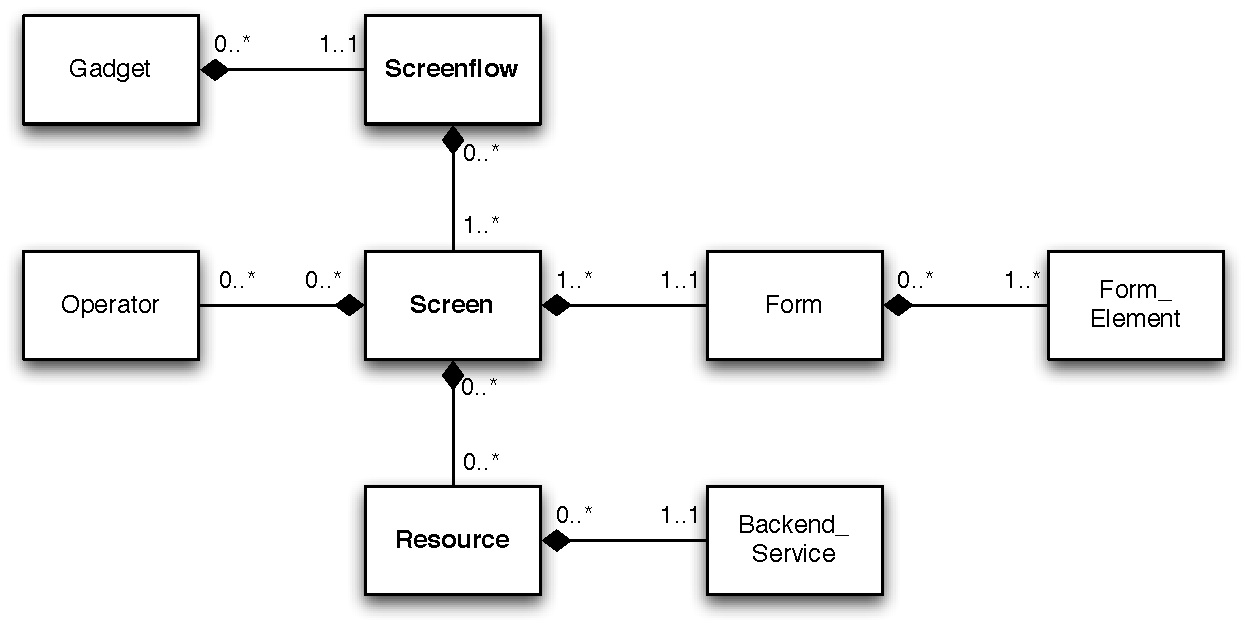
\includegraphics[scale=.66]{images/uml_composition.pdf}
    \caption{Important composition relationships within the FAST conceptual model}
    \label{fig:uml_composition}
  \end{center}
\end{figure}

Figure~\ref{fig:uml_screen_component} looks closer at the features of individual screens. These are forms, resources and operators, which are all specialisations of the general \emph{screen component} concept. Each such screen component may or may not have an action or trigger associated with them, which declaratively define their behaviour in terms of their own functionality or functionality they can trigger in other building blocks.

\begin{figure}
  \begin{center}
    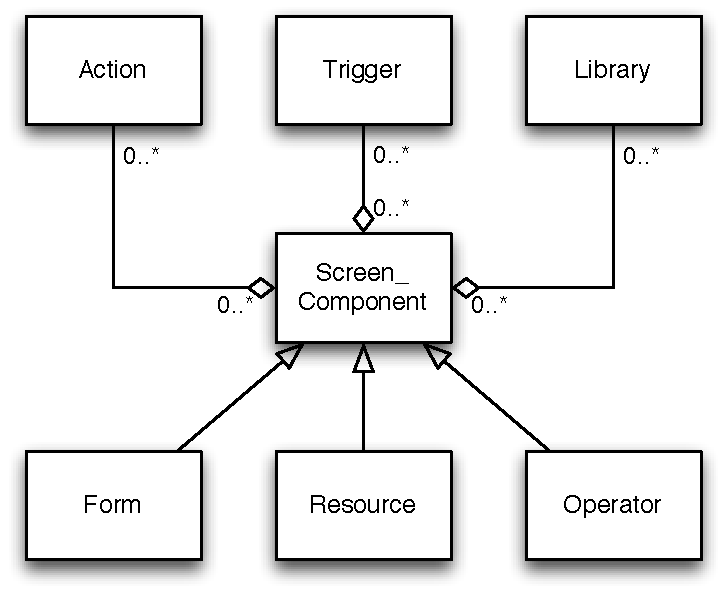
\includegraphics[scale=.66]{images/uml_screen_component.pdf}
    \caption{Aggregation of screen components}
    \label{fig:uml_screen_component}
  \end{center}
\end{figure}

Regarding their implementation, different kinds of building blocks in FAST can either be defined hard-coded as a piece of source code, or they can be defined declaratively in the terms of the FAST ontology (using pipes, operators, etc.). In the former case, a building block such as a screen would have been implemented and added to the FAST platform by an engineer, whereas in the latter case, ordinary users of the FAST platform would have assembled the building block using the tools available in the GVS\footnote{At this moment, only screens can be assembled in the GVS. Forms may or may not be editable in the GVS in the future. Other kinds of building blocks are not currently planned to be editable.}. This principle is reflected in Fig.~\ref{fig:uml_definition}, showing how certain kinds of building blocks aggregate either a \texttt{Definition} or \texttt{Code}, whereas other kinds of building blocks are always hard-coded. It should be noted that, in theory, there is no reason why not any kind of building block could be defined either way. However, the concrete set of building blocks which can be defined declaratively or in code is changing dynamically according to the current state and plans of the FAST project. The situation depicted in Fig.~\ref{fig:uml_definition} --- \texttt{Screen} and any kind of \texttt{Screen\_Component} can be defined in code, whereas only \texttt{Screen} and \texttt{Form} can be defined declaratively --- reflects the status at M24 of the project. 

\begin{figure}
  \begin{center}
    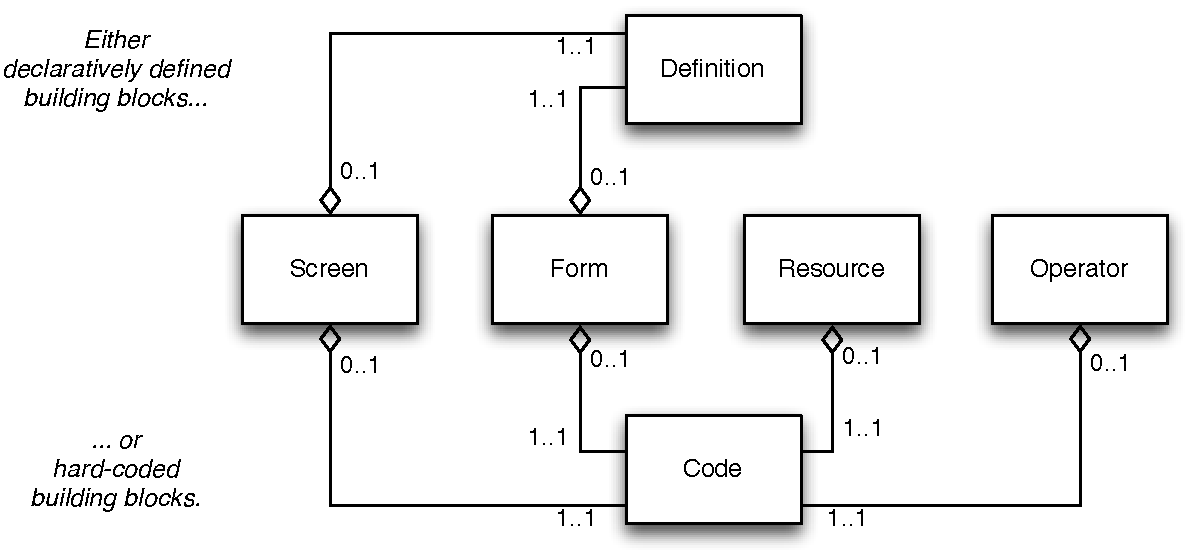
\includegraphics[scale=.66]{images/uml_definition.pdf}
    \caption{Building blocks have either code or are defined declaratively}
    \label{fig:uml_definition}
  \end{center}
\end{figure}

Figure~\ref{fig:uml_condition} illustrates how different building blocks relate to the concepts of pre- and post-conditions. While all building blocks can essentially have such conditions, only screens and screen flows directly aggregate both kinds of conditions. However, in the case of the three different kinds of screen components (form, resource and operator), the relation to a pre-condition is only established through their actions, which represent their basic functionality. For all building blocks, both pre- and post-conditions are entirely optional.

\begin{figure}
  \begin{center}
    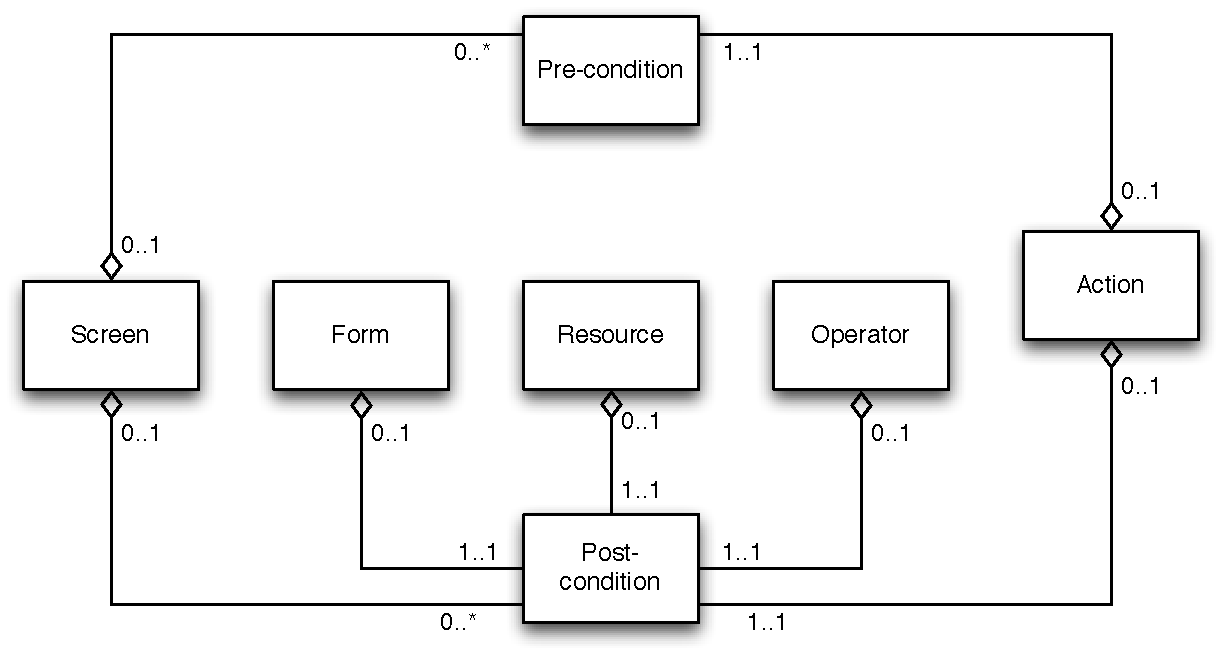
\includegraphics[scale=.66]{images/uml_condition.pdf}
    \caption{Building blocks with pre- and post-conditions}
    \label{fig:uml_condition}
  \end{center}
\end{figure}



% subsubsection term_relations_within_the_conceptual_model (end)

\subsection{Integration} % (fold)
\label{sub:integration}

In this section we will investigate a number of established ontologies which cover part of the requirements laid out in the specification document, as well as the glossary of terms from the conceptualisation stage. In particular, we will look at the Dublin Core metadata specification, the Friend of a Friend (FOAF) ontology, Semantically Interlinked Online Communities (SIOC)  and Common Tag. 
The outcome of the integration process is the living \emph{integration document} at \ref{ssub:integration_document}.

\subsubsection{Dublin Core} % (fold)
\label{ssub:dublin_core}

Dublin Core (DC) is a set of metadata elements for describing online resources in order to support indexing, searching and finding them. Typical examples of terms from DC are \emph{title}, \emph{creator}, \emph{subject}, \emph{description}, \emph{date} or \emph{rights}. In principle, DC can be applied to a wide range of resources, but is typically used in the context of describing media (textual documents, video, sound or image). The initial work on DC was done at an invitational workshop in Dublin, Ohio, US (hence the name) in 1995. Since then, several revisions and extensions have been applied to the vocabulary.

While it is possible to express DC in plain HTML, the more widely used language is probably RDF. The original 15 terms were all properties defined in the DC elements namespace (\url{http://purl.org/dc/elements/1.1/}, short \texttt{dc}). The properties were not formally defined with respect to their range and domain, or whether they are object or datatype properties. However, the assumption was that the values for each property would always be literals, as opposed to complex values represented by a URI. More recently, the DC elements namespace has been declared legacy and is now superseded by the DC terms namespace (\url{http://purl.org/dc/terms/}, short \texttt{dcterms})~\cite{dcterms2008}, which includes more precise re-definitions of all 15 original terms, as well as a number of new terms (resulting in a total of 55 terms). This new iteration of DC now provides the facility to use structured values for properties and specifies what type these values will have. E.g., the property \texttt{dcterms:creator} now supersedes the original \texttt{dc:creator} and specifies that its value has the type \texttt{dcterms:Agent}.

In order to reconcile with the simplicity of the original, flat DC elements and the newer, more structured DC terms, DC also includes the so-called ``DumbDown'' principle, which basically says that structured values of DC terms should always carry a literal description as well, in order to cater for ``dumb'' agents processing the data. These literals should be expressed using properties such as \emph{rdfs:label} or \emph{rdf:value}.

\begin{figure}
  \begin{center}
    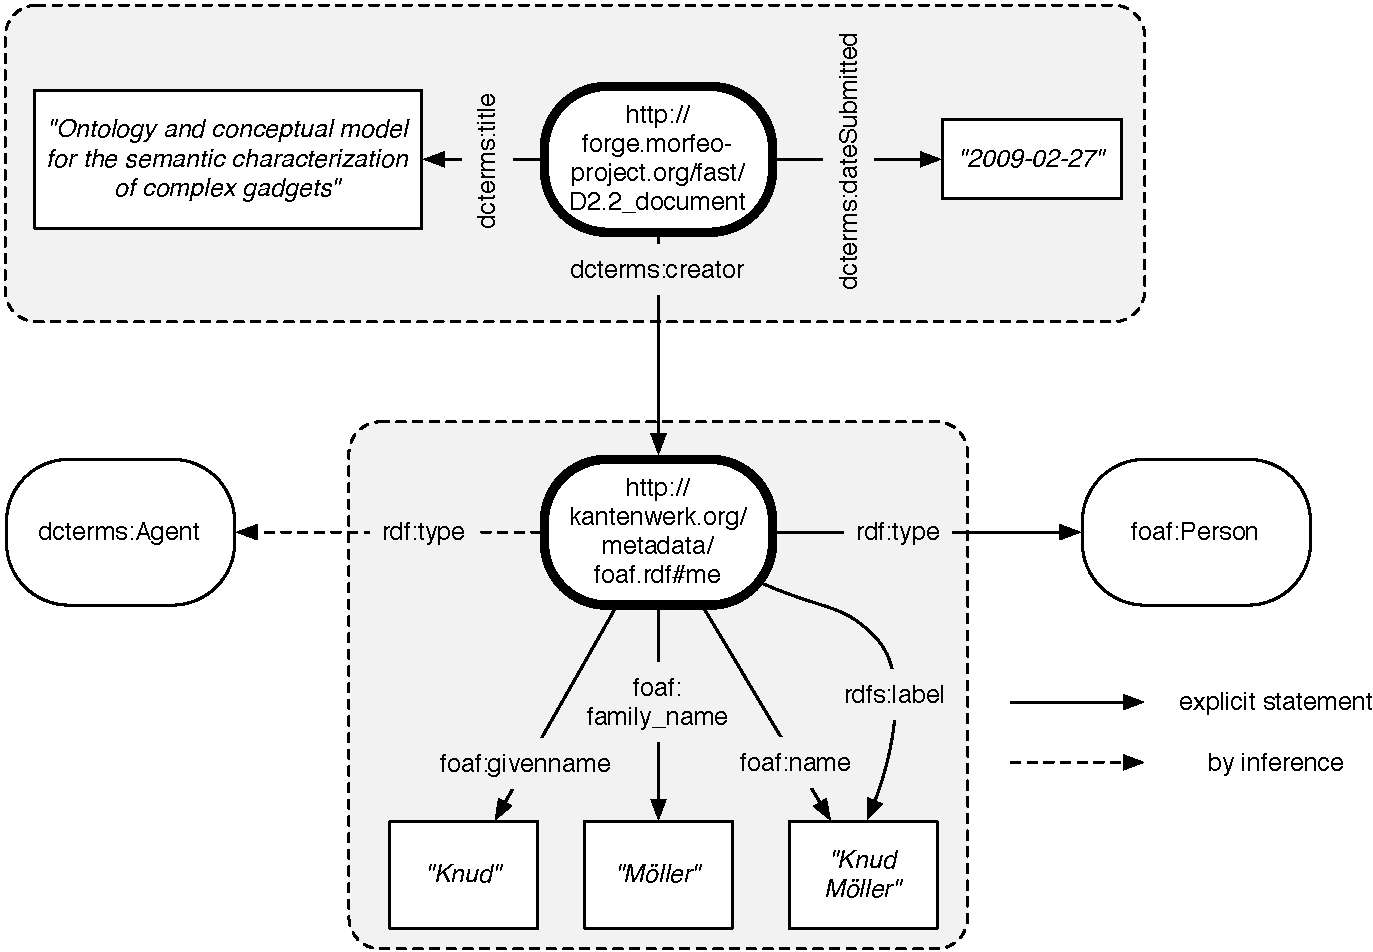
\includegraphics[width=\linewidth]{images/dcterms_example.pdf}
    \caption{Example of Dublin Core data}
    \label{fig:dcterms_example}
  \end{center}
\end{figure}

Because of the open nature of the RDF model and the open-world assumption usually applied for RDFS and OWL, it is possible to integrate DC with other ontologies such as FOAF. E.g., it is possible and good practice to make a statement saying that the \texttt{dcterms:creator} of a document is an instance of \texttt{foaf:Person}. By inference following from the DC terms specification, this person would then also be a \texttt{dcterms:Agent}. This scenario is illustrated in Fig.~\ref{fig:dcterms_example}. A similar, but slightly out-dated example is given in \url{http://dublincore.org/documents/dcq-rdf-xml/}.

Looking at the requirements specification document, DC can be integrated into the FAST gadget ontology in many ways. A lot of the metadata needs for screens, screenflows and their components are identical to those of the media resources originally intended by DC. For this reason, many properties such as \texttt{title}, \texttt{creator}, \texttt{rights} or various \texttt{date} properties can be used directly (more details in the integration document). 
% subsubsection dublin_core (end)

\subsubsection{FOAF} % (fold)
\label{ssub:foaf}

The Friend of a Friend vocabulary is a simple ontology which main purpose to describe people --- represented as instances of the \texttt{foaf:Person} class --- in terms of their contact information, interests, or Web presence. More importantly, however, is the fact that FOAF provides some simple terms for specifying who knows who (using the propery \texttt{foaf:knows}), thereby effectively allowing to build a social network of people. There is no such thing as a centralised FOAF service to which people have to sign up. Instead, each person can maintain and host their own FOAF description (often in the form of a \emph{FOAF file}), or use one of many external services which provide this functionality, such as LiveJournal, TypePad, Vox, Hi5, etc., thus making the FOAF network a truly decentralised social network. Figure ~\ref{fig:foaf_example} depicts an excerpt of some typical FOAF files, describing two people called ``Knud M\"oller'' and ``Andreas Harth'', including the fact that Knud knows Andreas.

\begin{figure}[ht]
  \begin{center}
    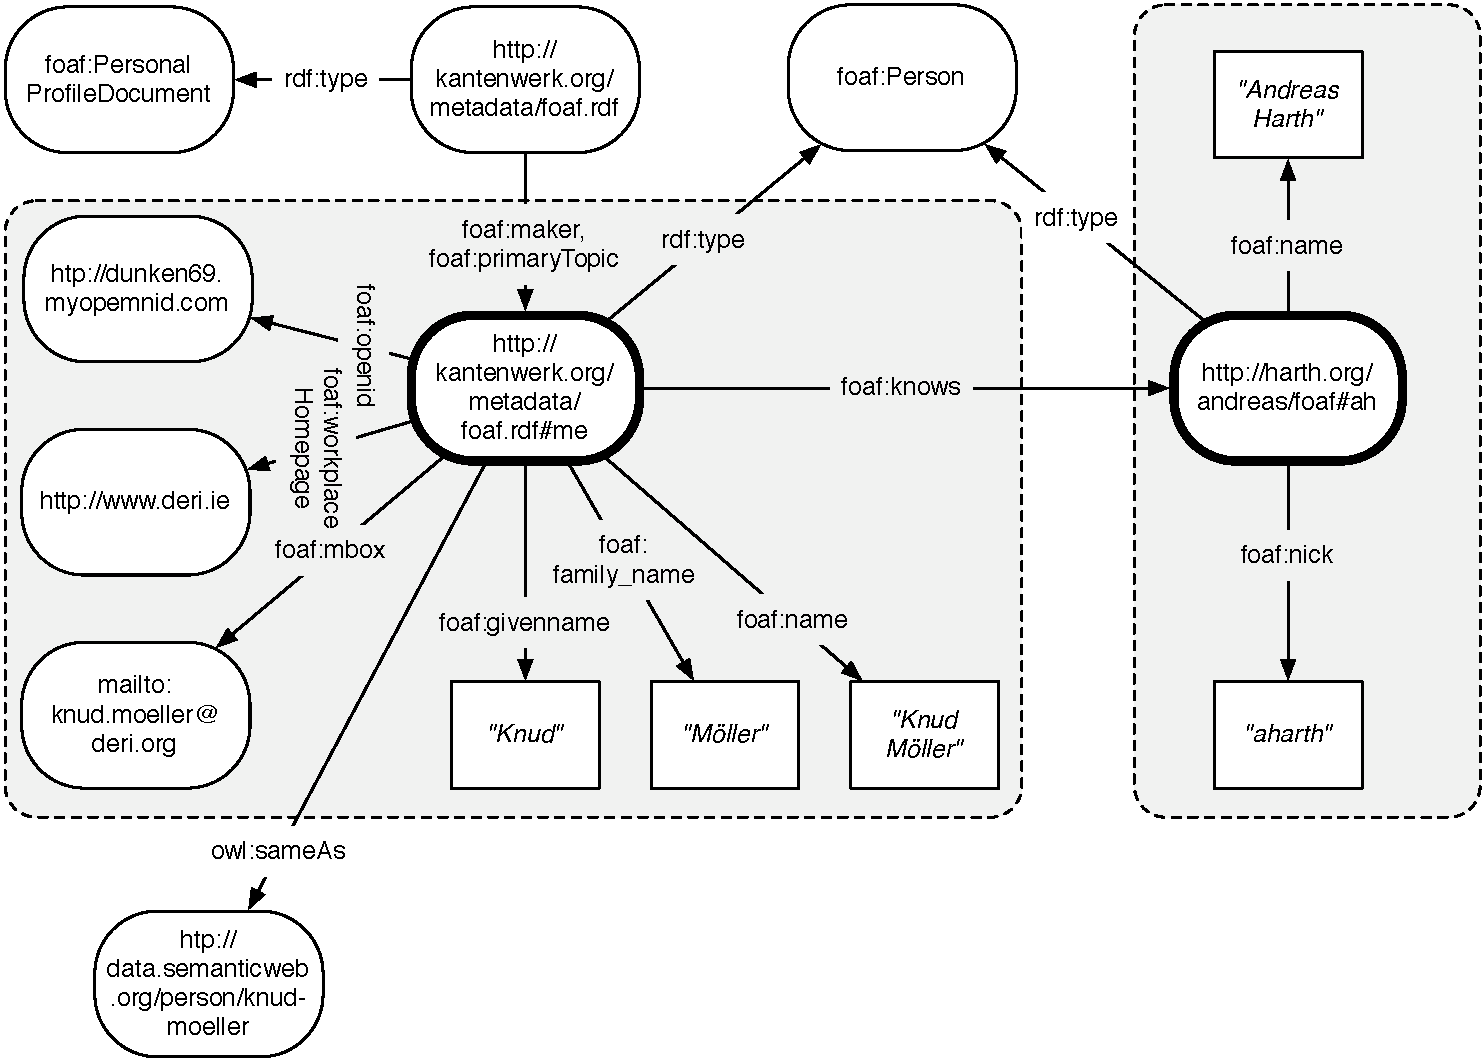
\includegraphics[width=\linewidth]{images/foaf_example.pdf}
    \caption{Example of FOAF data}
    \label{fig:foaf_example}
  \end{center}
\end{figure}

FOAF has been \emph{``evolving gradually since its creation in mid-2000''}~\cite{brickley2004foaf}. Over the years, it attracted a lot of attention and has become one of the major successes of the Semantic Web. Compared to most other ontologies or vocabularies, it has received a much higher uptake, with the number of FOAF files on the internet probably numbering tens of millions now. Its popularity in the community and beyond is also underlined by the fact that many other ontologies are integrating FOAF in order to represent basic information regarding people, or they are using it as a point of reference and extend the basic FOAF classes and properties for their own needs. Examples for this kind of integration are the increasingly popular SIOC (Semantically-Interlinked Online Communities) ontology~\cite{breslin2005communitiesEswc}, which uses FOAF description to unify identities in different online communities, or the Semantic Web Conference ontology~\cite{moeller2007dogfood}, where conference attendees or authors are represented as FOAF person instances.

The specification document of the FAST ontology defines that part of the purpose of the ontology is ``the description of users and user profiles''. The most obvious solution for implementing this requirement is to integrate the FAST ontology with FOAF. This means that each user of FAST would be modelled as a \texttt{foaf:Person}. A lot of the basic necessities in terms of user profile information is covered by properties defined in FOAF (names, contact details, interests, user pictures, etc.) and could therefore be used as is. In other cases, rather generic FOAF terms might be good starting points for extension towards more specific needs that occur in FAST. The icons of various components in the GVS may serve as an example here: the relation that holds between an icon and the thing X of which it is an icon could be described as ``the icon depicts X''. FOAF provides the property \texttt{depiction} to express this general relation. However, \texttt{hasIcon} (our property for saying that something is the icon of a thing) can be considered a specialisation of this, and so we will say that \texttt{fgo:hasIcon} is a specialisation of \texttt{foaf:depiction}. In terms of RDFS, we will say that \texttt{<fgo:hasIcon> <rdfs:subPropertyOf> <foaf:depiction>}.
% subsubsection foaf (end)

\subsubsection{SIOC} % (fold)
\label{ssub:sioc}

Another vocabulary that is gaining a lot of uptake and support on the Semantic Web is SIOC, which received additional weight when it became a W3C member submission in 2007. The basic idea behind SIOC is that there is an abstract model behind all online community sites which contain an aspect of discussion between members, be it forum sites, discussion boards, blogs, wikis, content management systems, mailing lists, etc. For each of those \emph{sites}, it can be said they contain discussion threads or \emph{fora}, which in turn contain \emph{posts}, which in turn can have \emph{comments}. Furthermore, each post or comment can have a \emph{topic} and a \emph{creator}, which can be a \emph{user} of the site. The authors of SIOC make a point of integrating the vocabulary with FOAF, e.g., by suggesting that a user of a site is in fact held by an instance of \texttt{foaf:Person} (the SIOC specification states that \texttt{sioc:User} is a sub-class of \texttt{foaf:OnlineAccount} \cite{sioc_spec2009}). An overview of the different classes and properties of SIOC is given in Fig.~\ref{fig:sioc_overview}.

\begin{figure}
  \begin{center}
    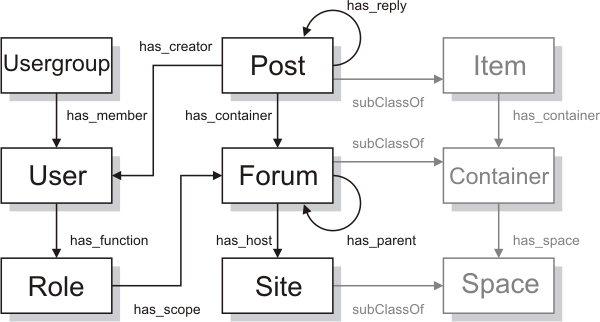
\includegraphics[width=0.8\linewidth]{images/sioc_overview}
    \caption{Overview of the SIOC ontology}
    \label{fig:sioc_overview}
  \end{center}
\end{figure}

From an implementation point of view, a particular site will use SIOC by exposing its internal data on request with the help of a SIOC exporter. Such components have been provided by various members in the SIOC developer community for different popular platforms, such as the WordPress blogging software, the Drupal CMS or the Twitter micro-blogging platform. The benefit that sites are creating for end users by using SIOC is that a common representation format and reference points such as authors and topics allow data from different sites to be integrated and thus browsed and searched together.

From the point of view of the FAST gadget ontology, the most interesting features of the vocabulary are the classes and properties it provides for modelling users of a site. We will use SIOC in combination with FOAF to model users and their profiles, as well as user groups, as specified in the requirements document. The discussion aspects of SIOC will not have an immediate use within the FAST platform. However, it is conceivable that collaborative features such as support for fora will be added to FAST at some point, which will lead to an extension of the requirements document. These additional requirements could then be fulfilled by the integration of further terms from SIOC.
% subsubsection sioc (end)

\subsubsection{Common Tag} % (fold)
\label{ssub:common_tag}

Common Tag\footnote{\url{http://www.commontag.org}, 24/01/2010} is an open format and initiative for conceptual tagging, which is developed and backed by a number of relevant players in the Web community, including Yahoo! and DERI. The basic idea of conceptual tagging is to address the problem of ambiguity in the meaning of tags (e.g., does ``jaguar'' mean the car, the animal or the operating system?) as it occurs in free-text tagging. Rather than relying on methods such as clustering, applied to a whole corpus of tagged resources, conceptual tagging intends to disambiguate a tag right from the moment it is used, by linking it to an unambiguous concept from vocabularies such as Dbpedia~\cite{Auer07dbpedia} (representing Wikipedia as linked data) or Freebase\footnote{\url{http://www.freebase.com/}}. E.g., in order to disambiguate ``cocoa'' as meaning the API, not the drink or plant, it would be represented as a resource (rather than a plain literal) and linked to the DBpedia resource \url{http://dbpedia.org/resource/Cocoa_%28API%29}.

Apart from facilitating the disambiguation of tags, Common Tag also allows to make further assertions about the nature of a tag, such as who applied it or when it was applied. As an example, List.~\ref{list:common_tag} shows how a blog post has been tagged on 20/01/2010 with ``cocoa'', meaning the API, not the drink or plant.

\singlespacing
\lstset{
	caption={Common Tag example --- disambiguating the tag ``cocoa''}, 
	label=list:common_tag,
	language=turtle
}
\begin{figure}
	\lstinputlisting{exampleCode/common_tag_example.ttl}
\end{figure}
\doublespacing

Within FAST, Common Tag is used to cover the tagging needs as specified in the ontology requirements specification, and in particular in order to define the domain context as specified in the annotation part of the glossary of terms (\texttt{Tag} and \texttt{hasDomainContext}).

% subsubsection common_tag (end)

\subsubsection{Integration Document} % (fold)
\label{ssub:integration_document}
%
This living document specifies how the terms from the glossary of terms are expressed using terms from the various ontologies presented in the previous sections.

\clearpage
\singlespacing
\begin{small}
\begin{longtable}{|p{3cm}|p{1.5cm}|p{3.5cm}|p{6.1cm}|}
\caption{\label{tab:integration_document}FAST Ontology integration document}\\
\hline
\rowcolor{fast@lightgrey}\textcolor{white}{\textbf{FAST Term}} & 
\textcolor{white}{\textbf{Integrated Ontology}} & 
\textcolor{white}{\textbf{Integrated Term}} & 
\textcolor{white}{\textbf{Comment}} \\ \hline
\endfirsthead
\multicolumn{4}{|c|}{\emph{\textbf{Classes}}} \\ \hline
\texttt{User} & FOAF & \texttt{foaf:Person} & A user in FAST will be modelled using a combination of FOAF and SIOC, so that an instance of \texttt{foaf:Person} will have an account on the FAST platform, represented by an instance of \texttt{sioc:User}, which is a subclass of \texttt{foaf:OnlineAccount}. The relationship is expressed using \texttt{foaf:holdsAccount}. This way of modelling directly follows the suggestions made by~\cite{sioc_related2007}.\\ \hline
\texttt{User} & SIOC & \texttt{sioc:User} & s.a.\\ \hline
\texttt{Image} & FOAF & \texttt{foaf:Image} & --- \\ \hline
\texttt{Tag} & Common Tag & \texttt{ctag:Tag} & Complex or conceptual tags are being used e.g. to model the domain context of resources.	 \\ \hline
\multicolumn{4}{|c|}{\emph{\textbf{Properties}}} \\ \hline
\texttt{hasLabel} & DC & \texttt{dcterms:title} & ---  \\ \hline
\texttt{hasCreator} & DC & \texttt{dcterms:creator} & DC defines the range of \texttt{dcterms:creator} to be \texttt{dcterms:Agent}. By inference, this obviously also holds within FAST. However, we will explicitly only use \texttt{foaf:Person} (also see Fig.~\ref{fig:dcterms_example}). \\ \hline
\texttt{hasDescription} & DC & \texttt{dcterms:description} & --- \\ \hline
\texttt{hasCreationDate} & DC & \texttt{dcterms:created} & Dates should be formatted according to ISO 8601~\cite{w3c_iso8601_1997}. \\ \hline
\texttt{hasRights} & DC & \texttt{dcterms:rights} & DC terms specify a number of classes to model the rights of resources. \texttt{dcterms:rights} links a resource to a \texttt{dcterms:RightsStatement}. The holder of the rights is specified by pointing from the resource to a \texttt{dcterms:Agent}, using the \texttt{dcterms:rightsHolder} property. \\ \hline
% \texttt{hasDomainContext} & DC & \texttt{dcterms:subject} & DC specifies that subject shoulds be non-literals. To allow simple tagging, we should represent tags as resources (\todo{common tag}). \\ \hline
\texttt{hasImage} & FOAF & \texttt{foaf:depiction} & The inverse \texttt{foaf:depicts} could also be used. \\ \hline
\texttt{hasIcon} & FOAF & sub-property of \texttt{foaf:depiction} & Icons are a specific kind of image, so we can relate this property to the \texttt{foaf:depiciton}. \\ \hline
\texttt{hasScreenshot} & FOAF & sub-property of \texttt{foaf:depiction} & Screenshots are a specific kind of image, so we can relate this property to the \texttt{foaf:depiciton}. \\ \hline
\texttt{hasName} & FOAF & \texttt{foaf:name} & Apart from \texttt{foaf:name}, which is used for the full name, more fine-grained properties such as \texttt{foaf:firstName}, \texttt{foaf:surname} or \texttt{foaf:title} and \texttt{foaf:nick} can be used as well. \\ \hline
\texttt{hasEmail} & FOAF & \texttt{foaf:mbox} & While \texttt{foaf:mbox} will be used for the plain e-mail address, \texttt{foaf:mbox\_sha1sum} will be used for an obfuscated version of the address. \\ \hline
\texttt{hasInterests} & FOAF & \texttt{foaf:interest} & --- \\ \hline
\texttt{hasUserName} & FOAF & \texttt{foaf:accountName} & --- \\ \hline
\texttt{hasDomainContext} & Common Tag & \texttt{ctag:tagged} & The domain context of a resource in FAST can be expressed as a complex tag. Further Common Tag properties can then be applied to make assertions about the tag itself. \\ \hline
\texttt{hasVersion} & DOAP & \texttt{doap:revision} & DOAP (Description of a Project) is a widely used vocabulary for basic annotation of software and other projects. \\ \hline
\end{longtable}
\end{small}
\doublespacing

%% subsubsection integration_document (end)
%
%% subsection integration (end)
%
%% section domain_analysis (end)
%
\clearpage
\section{The FAST Gadget Ontology} % (fold)
\label{sec:ontology}

While the previous section discussed the various steps preceding the definition of the actual ontology according to our chosen development methodology, this section focusses on concrete usage of the FAST gadget ontology in an RDFS/OWL environment. As a point of reference, an overview of all concrete classes will be given in Sect.~\ref{sub:ontology_overview}, followed by a number of sections detailing concrete aspects of the usage of the FAST gadget ontology.

\subsection{Ontology Overview} % (fold)
\label{sub:ontology_overview}

This section gives a general, birds-eye-view of the ontology in terms of its classes and properties. Fig.~\ref{fig:ontology_uml} shows all classes in their subsumption hierarchy as a UML diagram, including the properties defining those classes as their domain. All \texttt{rdfs:subClassOf}/\texttt{rdfs:superClassOf} relations are modelled with the subsumption arrow, while \texttt{owl:union\_of} relations are modelled using the filled composition diamond.
A more detailed list of classes and properties, complete with human-readable comments and documentation can be found in the back of the document in App.~\ref{sec:ontology_terms}, while the complete ontology code in OWL is given in App.~\ref{sec:ontology_code}.

\begin{figure}
  \begin{center}
    \includegraphics[width=\linewidth]{images/fgo_uml_diagram}
    \caption{FAST Gadget Class Hierarchy}
    \label{fig:ontology_uml}
  \end{center}
\end{figure}


% subsection ontology_overview (end)

\subsection{Levels of Representation} % (fold)
\label{sub:classes_instances_and_templates}

In FAST, resources (gadgets, screenflows, screens and their components) exist in different stages throughout their lifecycle. Moving top-down from the high-level conceptual description to gadgets in use at runtime, the following differences can be made in terms of the level of instantiation:

\begin{itemize}
	\item \textbf{Abstract Class Level}: At this level, resources are defined on a categorical level, differentiating between the various kinds of things that are relevant in FAST, as fundamental classes such as screens, forms or resources (see Sect.~\ref{sub:conceptualisation}). These are implemented technically as classes in OWL.
	\item \textbf{Prototypical Component Definition}: When a user of the FAST GVS is building a new screenflow or screen, they do so by combining existing building blocks and configuring them. These building blocks are not the fundamental classes of FAST, but instead they are specific instances of those classes. In other words, users do not combine the idea of a screen with the idea of a service, but instead they combine the specific ``Log In Screen'' with the ``Amazon Web Service''. Technically, these concrete building blocks are implemented as instances of the fundamental classes, specified by asserting particular settings such as label or icons, pre- and post-conditions, etc.
	\item \textbf{Instantiation within a Screenflow at Design-time}: Once a user selects a specific building block in the GVS and adds it to their new screen or screenflow project, they are in principle again instantiating from a conceptual to a concrete level: from the ``Log In Screen'' as such to a particular log in screen as used in that particular screenflow. Also in this stage, resources are implemented technically as instances.
	\item \textbf{Runtime}: At the final level of instantiation, the screenflow has been packaged as a gadget, deployed to a gadget platform and is now being used by an end-user. At this level, all gadget components exist only in the form of Web standards compliant code (HTML, JavaScript, CSS). For performance reasons, the FAST catalogue transforms any metadata still necessary, as well as definitions for screen pre- and post-conditions, from their original RDF representations into the JavaScript Object Notation (JSON)\footnote{\url{http://www.json.org/}}. The JSON structures used at this level are described in \cite{palaghita2010catalogue_manual}. At this level, the resources that make up the gadget have moved out of the scope of the FAST platform and therefore out of the scope of this deliverable.
\end{itemize}

\begin{figure}
  \begin{center}
    \includegraphics[width=\linewidth]{images/classes_templates_instances.pdf}
    \caption{Different levels of representation of FAST building blocks}
    \label{fig:classes_templates}
  \end{center}
\end{figure}

When implementing these four stages, as illustrated in Fig.~\ref{fig:classes_templates}, in OWL DL semantics, we are faced with an immediate problem. Conceptually, we would like to say that $Screen$ is a class, i.e., the set of all screens. As argued above, $LogInScreen$ would then be an instance of $Screen$ ($LogInScreen \subset Screen$), while a particular $LogInScreen_x$ in a particular screenflow would again be an instance of $LogInScreen$ ($LogInScreen_x \subset LogInScreen$). However, unless we want to move into OWL Full semantics, classes cannot be used as instances at the same time, so we cannot use this modelling approach. Furthermore, when we instantiate a resource such as a screen within a particular screenflow, we want to imply that the new instance ($LogInScreen_x$) has the same features such as label, icon or conditions, as $LogInScreen$. In other words, what we really require is a something like a \emph{copy} or a \emph{clone} of the original $LogInScreen$. 

\subsubsection{Prototypes} % (fold)
\label{ssub:prototypes}

% subsubsection prototypes (end)

Neither OWL nor RDFS semantics offer functionality to represent a relationship such as the clone of a resource formally. However, we can find inspiration for this kind of semantics in other areas, such as programming languages, and more particularly in object-oriented programming languages (OO). In OO, there is a general dichotomy between \emph{class-based} languages and \emph{prototype-based} languages. Both paradigms address the issue of defining similarity between objects, but do so in a different way. The class-based paradigm requires an a-priori classification and categorisation of the world (the class hierarchy), into which individual objects (the instances) are then grouped. All instances of a class inherit the attributes and functionality of the class. Changing this behaviour usually involves changing the class. Prototype-based languages, on the other hand, do not assume prior categorisations. Instead, one starts with specific examples and then generalises from there. These languages do not show a class vs. instance distinction. Instead, all objects have the same status, and new objects can be \emph{cloned} from other objects, which function as \emph{prototypical objects} in this situation. The new object (or clone) will inherit all attributes and functionality from the prototype. Changing behaviour can be done on each object individually.

\todo{Rewrite this whole section with focus on prototypes, prototype theory, prototype-based programming, etc.}

\cite{Taivalsaari96classes_vs_prototypes}

\begin{itemize}
	\item in a prototypical programming language, creating an object from a prototype means to clone it --- copy all its attributes\footnote{Whether or not this is true copy or merely a pointer is implementation-dependant. This is more or less transparent for the user.}
	\item in RDF, what would ``all its attributes'' mean?
	\item this is the old question of what constitutes an object in RDF
	\item should we use the minimal self-contained graph \cite{Tummarello:2008kl}?
	\item maybe some other named graph? But the RDF model doesn't feature named graphs
	\item let's just assume some unspecified ``object graph'' for now --- the exact definition of the object graph is application dependent. In FAST, it is actually always known which triples constitute the object graph of a building block.
	\item so, now that we can say that the prototype object, identified by its URI (we therefore call it $P_{URI}$), is defined by its object graph, we can define the relation between the prototype and its clone ($C_{URI}$) as follows:
\end{itemize}

\begin{equation}
S:= \begin{cases}
i = 0..M,\quad j =0..N  & \text{for }M >N \\
i=0..M,\quad j=0..M & \text{for }N > M
\end{cases}
\end{equation}


For this reason, we introduce the concept of \emph{templates for RDF instances} in FAST. Templates are similar to the notion of prototypes in programming languages such as JavaScript. One resource (e.g., $LogInScreen$) will play the role of a \emph{template}, while the other resource (e.g., $LogInScreen_x$) will be called a \emph{copy}. Conceptually, copying a resource involves the following steps:
\begin{inparaenum}[(i)]
	\item Defining a named graph $G_1$ that contains all statements about this resource considered to be relevant.
	\item Creating a second graph $G_2$ with copies of all statements in $G_1$.
	\item During this copying process, the identifiers for the main resource and certain other resources in the graph will be changed from $I_{template}$ to $I_{copy}$.
\end{inparaenum}	
In practice, this procedure can be implemented using a SPARQL CONSTRUCT query, where the WHERE clause defines the graph pattern of the template, and the CONSTRUCT query will build the copy from it. The corresponding data on all three levels is shown in List.~\ref{list:prototyping}, using TriG syntax~\cite{bizer2004trig} (an extension of Turtle syntax for named graphs).

\singlespacing
\lstset{
	caption={Prototyping example --- different levels of representation of a FAST screen (code)}, 
	label=list:prototyping,
	language=turtle
}
\begin{figure}
	\lstinputlisting{exampleCode/prototypeExample.ttl}
\end{figure}
\doublespacing

Figure \ref{fig:prototype_example_graph} illustrates the same example graphically, using different colours to represent the two different graphs: the red graph $G_1$ in the background represents the original template resource, whereas the green graph $G_2$ in the front in represents the resource copy as it would be used in a concrete screen flow. \texttt{catalogue:LoginScreen} $\subset I_{template}$ has been changed to \texttt{catalogue:LoginScreen\_74382} $\subset I_{copy}$.

\begin{figure}
  \begin{center}
    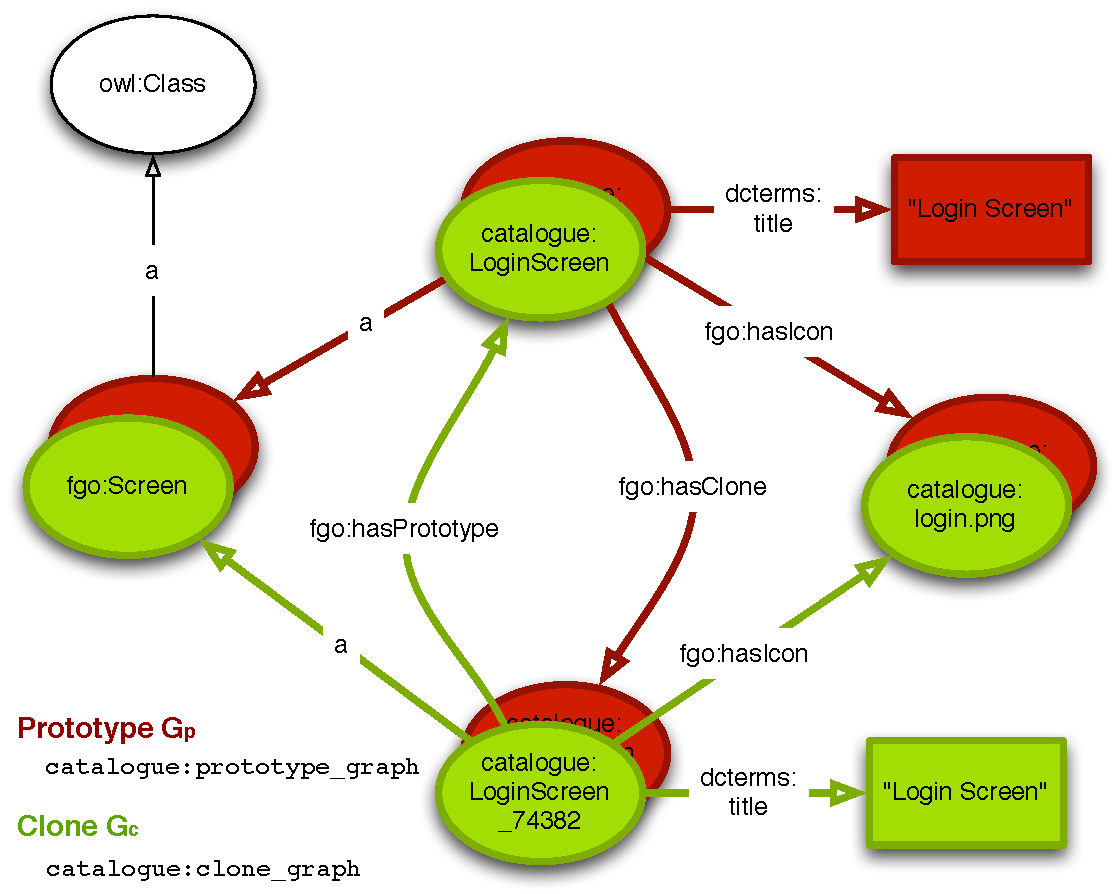
\includegraphics[width=.75\linewidth]{images/prototypeExample.pdf}
    \caption{Prototyping example --- different levels of representation of a FAST screen (diagram)}
    \label{fig:prototype_example_graph}
  \end{center}
\end{figure}


It should be pointed out that the term \emph{RDF template} has been used before, but with a different meaning. \cite{davis2003rdf_template} use the term in analogy to XSLT, but acting on an RDF graph rather than an XML tree. \cite{kawamoto2006kawawiki} present a semantic wiki, where templates help non-technical users to create semantic descriptions. 
% subsection classes_instances_and_templates (end)

\subsection{Basic Annotation} % (fold)
\label{sub:basic_annotation}

In this section, we will present the use of some basic resource annotation properties in FAST. In general, since screenflows, screens and their components are sub-classes of \htmlref{\texttt{fgo:Resource}}{subs:Resource}, all properties defined to have a domain of \htmlref{\texttt{fgo:Resource}}{subs:Resource} should be used. In addition, a number of terms from external ontologies should also be used to annotate resources. Note that all of these annotations are valid both for the prototypical component definitions (templates) and the design time instances (copies). A detailed description of all terms from the FAST gadget ontology namespace can be found in Sect.~\ref{sec:ontology_terms} of this document.

\singlespacing
\lstset{
	caption={Example of basic annotation of a FAST resource}, 
	label=list:basic_annotation,
	language=turtle
}
\begin{figure}
	\lstinputlisting{exampleCode/screen_example.ttl}
\end{figure}
\doublespacing

% subsection basic_annotation (end)

\subsection{FAST Users} % (fold)
\label{sub:fast_users}

In modelling resources in FAST, the kind of users that are relevant are the users of the FAST tools themselves (i.e., the GVS), as opposed to end users of the gadgets. The following List.~\ref{list:user} shows how an individual user is modelled, using terminology from the FOAF and SIOC vocabularies.

\singlespacing
\lstset{
	caption={Basic description of a user in FAST}, 
	label=list:user,
	language=turtle
}
\begin{figure}
	\lstinputlisting{exampleCode/user_example_01.ttl}
\end{figure}
\doublespacing

Once a user has been defined in this way, they can for example be used to specify the creators of individual screen and screenflow resources, as shown in List.~\ref{list:creator}. This kind of creation metadata is being added to other metadata as shown in Sect.~\ref{sub:basic_annotation}.

\singlespacing
\lstset{
	caption={Modelling the creator of a resource}, 
	label=list:creator,
	language=turtle
}
\begin{figure}
	\lstinputlisting{exampleCode/user_example_02.ttl}
\end{figure}
\doublespacing


% subsection fast_users (end)

\subsection{Defining Pre- and Post-conditions} % (fold)
\label{sub:defining_pre_and_post_conditions}

The facts which define the pre- and post-conditions of screens and screenflows in FAST are modelled as individual RDF triples. In effect, this means that conditions, which are sets of facts, are modelled as graph patterns using SPARQL notation \cite{sparql2008spec}. E.g., a simple pre-condition such as \emph{``There has to be a user''} could be expressed as in List.~\ref{ex:simple_precondition}. Literally, this very simple pattern means \emph{``a variable ?user is of type sioc:User''}. In logical terms, it means something along the lines of \emph{``there exists a sioc:User''}. In order to determine if this  pre-condition can be fulfilled, it needs to be executed against the RDF graph in question. This graph could for example consist of the set of post-conditions of all screens currently available on the canvas.

\singlespacing
\lstset{
	caption={Simple pre-condition}, 
	label=ex:simple_precondition,
	language=sparql
}
\begin{figure}
\begin{lstlisting}
	?user a sioc:User .
\end{lstlisting}
\end{figure}
\doublespacing

Post-conditions are expressed in a similar fashion. In the prototypical phase (i.e., as part of templates), post-condition patterns have variables in the same way as pre-condition patterns. When a building block is copied to the canvas, the pattern needs to be materialised. To do this, each variable will be replaced with a randomly generated URI or blank node. At runtime, variables are then replaced with actual values once the screen for which the post-condition holds has been executed. As an example, consider the post-condition of a login screen. In natural language, it could be \emph{``Once the login process has finished, there will be a user object''}. Using the same notation as before, this could be expressed as shown in List.~\ref{ex:postcondition}, extended with some additional facts (\emph{``There is a user object which has an account name. There is also a person which has a name, and which has the user object as an online account.''}).

\singlespacing
\lstset{
	caption={Post-condition at the prototypical stage}, 
	label=ex:postcondition,
	language=sparql
}
\begin{figure}
\begin{lstlisting}
	?user a sioc:User ;
	      foaf:accountName ?account_name .
	?person a foaf:Person ;
	      foaf:holdsAccount ?user ;
	      foaf:name ?person_name .
\end{lstlisting}
\end{figure}
\doublespacing

Once added to the canvas in the GVS (``instantiated at design time''), each variable is then replaced with a blank node identifier, as shown in example~\ref{ex:postcondition_canvas}. This is necessary because, while variables are available in SPARQL, they cannot be represented directly in RDF. The pre-condition in example~\ref{ex:simple_precondition} could now be matched successfully as a SPARQL query against the canvas graph.

\singlespacing
\lstset{
	caption={Post-condition as instantiated during design time (on the FAST GVS canvas)}, 
	label=ex:postcondition_canvas,
	language=sparql
}
\begin{figure}
\begin{lstlisting}
	_:b0 a sioc:User ;
	      foaf:accountName _:b1 .
	_:b2 a foaf:Person ;
	      foaf:holdsAccount _:b0 ;
	      foaf:name _:b3 .
\end{lstlisting}
\end{figure}
\doublespacing

Finally, during runtime, the post-condition's variables would be replaced with the actual values of the user which completed the login screen (``instantiated during runtime''). E.g., this could result in a graph such as in example~\ref{ex:postcondition_runtime}. However, in the current implementation of FAST, gadgets do not use an RDF representation of facts at runtime, but instead a translation of the facts into the JSON format.

\singlespacing
\lstset{
	caption={Post-condition during runtime}, 
	label=ex:postcondition_runtime,
	language=sparql
}
\begin{figure}
\begin{lstlisting}
	<http://fast.org/gvs/knud> a sioc:User ;
	      foaf:accountName "dunk" .
	<http://kantenwerk.org/metadata/foaf.rdf#me> a foaf:Person ;
	      foaf:holdsAccount <http://fast.org/gvs/knud> ;
	      foaf:name "Knud Moeller" .
\end{lstlisting}
\end{figure}
\doublespacing

Regarding the representation of condition graph patterns and their linking to building blocks in the FAST backend, two parallel approaches are being followed. Each graph pattern is 
\begin{inparaenum}[(i)]
	\item represented as a named graph which is linked from an \texttt{fgo:Condition} using the \texttt{fgo:hasPattern} property, and
	\item as a string, linked from the condition using the \texttt{fgo:hasPatternString} property. This second approach is followed for convenient rendering in user interfaces and to allow optional support the use of a triple store without support for named graphs.
\end{inparaenum}
Each such condition will be linked to a screen or screenflow using either the \texttt{fgo:has\-PreCondition} or \texttt{fgo:has\-Post\-Condition} property. A concrete example of this principle is given in List.~\ref{list:post_condition}.

\singlespacing
\lstset{
	caption={Linking screens to conditions}, 
	label=list:post_condition,
	language=turtle
}
\begin{figure}
	\lstinputlisting{exampleCode/post_condition_example.ttl}
\end{figure}
\doublespacing


Since SPARQL has no direct support for negation, and since there is a need to allow screens to remove facts from the canvas graph as well as adding them, both pre- and post-conditions can be modelled to be either \emph{positive} or \emph{negative} using the \texttt{fgo:isPositive} property. For pre-conditions, the interpretation of \emph{positive} is that the condition must hold, while \emph{negative} means that the negation of the condition must hold. For post-conditions, \emph{positive} leads to the instantiated condition being added to the canvas, while \emph{negative} will remove the instantiated condition. These interpretations are summarised in Tab.~\ref{tab:is_positive}.

\begin{table}[ht]
	\caption{Different semantics for \texttt{isPositive}}
	\label{tab:is_positive}
	\begin{center}
		
		\begin{tabular}{lcc}
			\toprule
			& \textbf{pre-condition} & \textbf{post-condition} \\ 
			\midrule
			\emph{isPositive: true} & condition must be fulfilled & condition instantiated\\ 
			\emph{isPositive: false} & $\neg$condition must be fulfilled & instantiated condition removed \\ 
			\bottomrule
		\end{tabular}
	\end{center}
\end{table}


% 
% \subsection{Instance Examples} % (fold)
% \label{sub:instance_examples}
% 
% \subsubsection{Complete Screen with Opaque Code} % (fold)
% \label{ssub:complete_screen}
% 
% \singlespacing
% \lstset{
% 	caption={Complete Screen with Opaque Code}, 
% 	label=list:screen_01
% }
% % \setlength\parindent{0in}
% % \begin{minipage}[t]{\textwidth}
% \lstinputlisting{exampleCode/01_screenExample.ttl}
% % \end{minipage}
% % \setlength\parindent{0.21in}
% \doublespacing
% 
% % subsubsection complete_screen (end)
% 
% \subsubsection{Complete Screen with Declarative Definition} % (fold)
% \label{ssub:complete_screen_with_declarative_definition}
% 
% \singlespacing
% \lstset{
% 	caption={Complete Screen with Declarative Definition}, 
% 	label=list:screen_02
% }
% % \setlength\parindent{0in}
% % \begin{minipage}[t]{\textwidth}
% \lstinputlisting{exampleCode/02_screenExample.ttl}
% % \end{minipage}
% % \setlength\parindent{0.21in}
% \doublespacing
% % subsubsection complete_screen_with_declarative_definition (end)
% 
% % subsection instance_examples (end)

\subsection{Conditions and Piping within Screens} % (fold)
\label{sub:piping_within_screens}

In year two of the FAST project, work has been started to extend the flexibility of the GVS to also include the creation of new screens from building blocks, as opposed to only assembling pre-made screens into screen flows. The gadget ontology supports this by modelling screen internals such as \emph{forms}, \emph{service resources} and \emph{operators}. Each of those building blocks can have their own pre- and post-conditions (either directly or through their \emph{actions}). However, while conditions on the screen/screen flow level are matched automatically and the flow of data is establish dynamically, on the screen-internal level this is defined explicitly through \emph{pipes}. Pipes are themselves components of a particular screen and connect matching post- and pre-conditions of other components in the same screen. 

\begin{figure}
  \begin{center}
    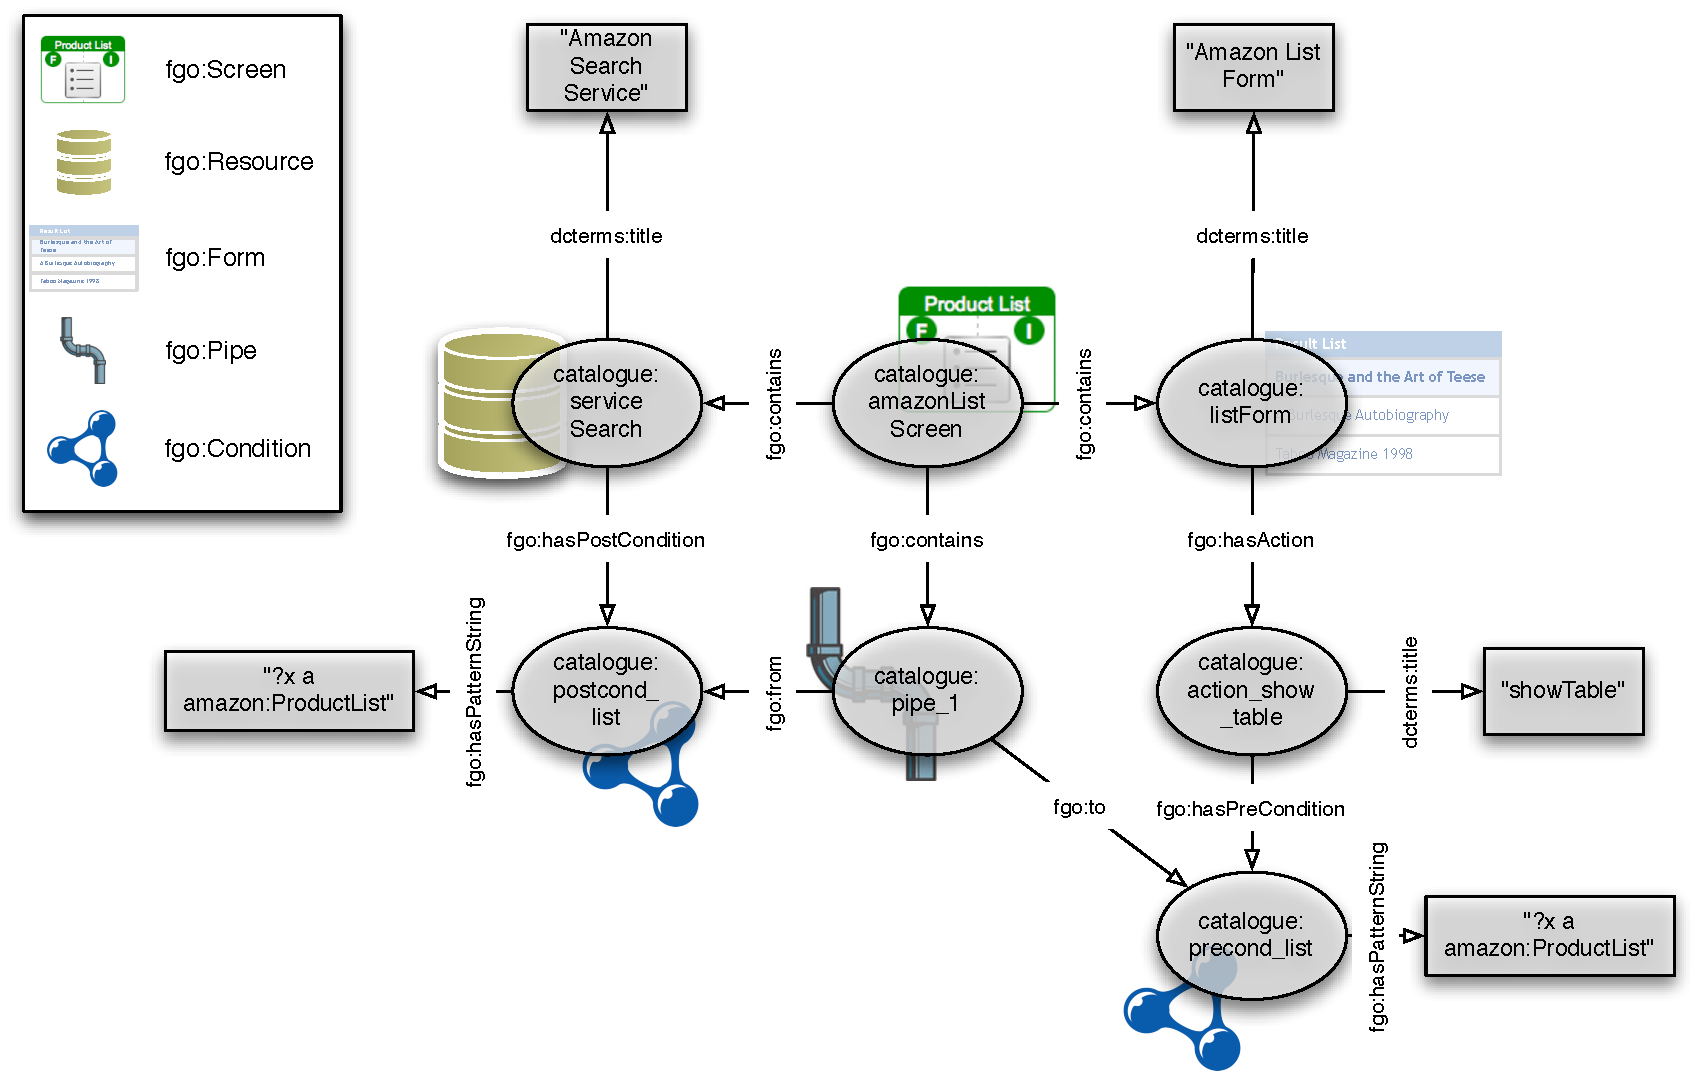
\includegraphics[width=\linewidth]{images/declarativeDefinitionExample.pdf}
    \caption{Explicit piping within a screen from a post- to a pre-condition (diagramme)}
    \label{fig:piping}
  \end{center}
\end{figure}

The concept of piping on this level of the FAST platform is illustrated graphically in Fig.~\ref{fig:piping}, and in code in List.~\ref{list:piping}\footnote{The example does not show a complete screen definition, but only the aspects which are relevant for this section.}. The screen is composed of (possibly among other things) a backend service resource, which wraps the Amazon search service, as well as a frontend Web form, which shows a list of Amazon products to the user. Additionally, the screen contains an instance of \texttt{fgo:Pipe}, which links the resource's post-condition (a product list) to the matching pre-condition of the form's ``showTable'' action. The desired functionality of this arrangement is that, whenever the service has returned a list of products in response to a search, this list will be piped to the form, where it will be displayed to the gadget's user.

\singlespacing
\lstset{
	caption={Explicit piping within a screen from a post- to a pre-condition (code)}, 
	label=list:piping,
	language=turtle
}
\begin{figure}
	\lstinputlisting{exampleCode/piping_example.ttl}
\end{figure}
\doublespacing


% subsection piping_within_screens (end)

\subsection{Extension towards Specific Domains} % (fold)
\label{sub:extension_towards_specific_domains}

While the FAST gadget ontology provides the framework and scaffolding for the formal description of complex gadgets, any  tailoring of a gadget or building block for a specific domain requires the integration of external domain ontologies. These ontologies can either be existing domain ontologies (e.g., the Good Relations ontology~\cite{Hepp:2008jr}\footnote{\url{http://www.heppnetz.de/projects/goodrelations/}} for e-Commerce) or ontologies which were purpose-built for FAST.
There are three main entry points at which external ontologies come into play:

\begin{itemize}
	\item \emph{Domain Contexts:} By providing a domain context for a screen (or any other FAST building block), it is possible to express what domain this resource is relevant for. Examples for domain contexts are ``medicine'', ``EU projects'', ``catering'', ``human resources'', ``books'', etc. As defined in the Integration Document in Sect.~\ref{ssub:integration_document}, we integrate the \texttt{ctag:tagged} property from the Common Tag vocabulary to define domain contexts as complex tags. As discussed in Sect.~\ref{ssub:common_tag}, one option for finding domain identifiers to be used with this property is the use of DBpedia identifiers such as \url{http://dbpedia.org/resource/Medicine} (DBpedia is a large RDF corpus automatically extracted from the info boxes of Wikipedia entries). This is now a widely used and recommended practice in the Semantic Web community. Similar corpora such as FreeBase could also be used. A concrete example of defining the domain context of the login screen to the Amazon service is given in List.~\ref{list:domain_context}, showing the use of \texttt{ctag:means} to disambiguate the meaning of the tag ``Amazon.com''.
	\item \emph{User Interests:} In the same way as domain contexts, a user's interests can be specified using DBpedia identifiers and structured tagging. Matching domain contexts to used interests, the GVS (through the catalogue) can then suggest relevant resources to the user.
	\item \emph{Pre- and Post-conditions:} In specifying pre- and post-conditions, terminology for an open-ended number of domains is necessary. While a number of classes will be reused quite often, very specific screens will require very specific vocabulary. We cannot, as part of the FAST project, provide vocabulary for all conceivable domains of discourse, and while also here DBpedia identifiers may be an option, often more precise terms will be needed.
\end{itemize}

\singlespacing
\lstset{
	caption={Defining a screen's domain context using the Common Tag vocabulary}, 
	label=list:domain_context,
	language=turtle
}
\begin{figure}
	\lstinputlisting{exampleCode/domain_context_example.ttl}
\end{figure}
\doublespacing


It should be added that for any given screenflow, the concrete definition of both domain context could be derived automatically from any semantic description which the backend services might have. While this might happen directly, without any transformation or mapping, this approach would be impractical in practice. The reason for this is that each backend service can potentially (and very probably) express its semantics in different ontologies or vocabularies, which would render the pre- and post-condition mechanism in FAST useless. Therefore, we assume that a mapping or mediation layer will ensure that the different semantics at the backend service level will be mapped to a common set of terms within the FAST platform. This problem is the topic of deliverable 2.4 in FAST~\cite{ambrus2010fast_mediation} and has also been discussed in \cite{Ambrus:2009it}.
% subsection extension_towards_specific_domains (end)

% section the_fast_gadget_ontology (end)

\clearpage
\section{Evaluation} % (fold)
\label{sec:evaluation}

The FAST ontology is continuously being evaluated through its direct and indirect employment in the implementation work packages WP3-5, as well as through an ongoing dialogue between the ontology designers and the platform implementers. The use case-based evaluation performed in WP6 provides additional input to this process. 
This kind of evaluation has lead to the gradual change, extension and adjustment of the documents produced in the different stages in the ontology development process, such as the glossary of terms in the conceptualisation phase, the integration document and the formal OWL ontology document. In addition to this kind of continuous evaluation we have also looked into other kinds of metrics ontology evaluation, as discussed in the following paragraphs.


\subsection{Usability as a General Design Principle} % (fold)
\label{sub:general_design_decisions}

Apart from ``hard'' metrics for the evaluation of ontologies, so-called ``soft'' factors for ontologies are relevant for facilitating better understanding by users and implementers, and therefore ultimately greater usability and uptake. \cite{moeller2009ontology_soft_skills} define five such soft factors as guidelines for ontology developers:

\singlespacing
\begin{itemize}
	\item \textbf{reuse external ontologies} to facilitate integration and compatibility,
	\item \textbf{avoid over-engineering} and keep the number of ontology terms down to reduce the cognitive load on implementers,
	\item \textbf{be a good Web citizen} by following the principles of linked data,
	\item \textbf{document well} to make it easy for implementers to understand and use the ontology correctly and
	\item \textbf{provide tool support} to ease the work-load involved in generating instance data.
\end{itemize}
\doublespacing

In the following, we will look at each of those guidelines and discuss how far the FAST gadget ontology fulfils them.

\subsubsection{Reuse of Existing Ontologies} % (fold)
\label{ssub:reuse_of_existing_ontologies}

An important aspect to consider when designing any ontology which is aimed to be used not only within a restricted institution or community is to reuse terms from existing ontologies and vocabularies as much as possible. Reuse serves the purpose of lowering the entry barrier for third parties to adopt the ontology --- if they can use familiar concepts and terms, they will be more inclined to try out something new. Equally important is the fact that reuse of terms facilitates data integration, which, after all, is one of the major goals of the Semantic Web at large.

Rather than reinventing the wheel in the various terms that have been defined in its requirement specification, the FAST gadget ontology integrates a number of well-established external ontologies. In particular, FOAF and SIOC are used to model tool users and developers, Dublin Core is applied for its general purpose annotation vocabulary and Common Tag is integrated to allow the modelling of a FAST resource's domain context as complex conceptual tags. Details are given in Sect.~\ref{sub:integration}.
% subsubsection reuse_of_existing_ontologies (end)

\subsubsection{Avoid Over-engineering} % (fold)
\label{ssub:avoid_of_over_engineering}

The concrete interpretation of this criterion depends to a large degree on the intended use case and user community of the ontology. For a large-scale undertaking spanning many domains, and where reasoning is in the centre of attention --- CyC\footnote{\url{http://cyc.com/cyc/opencyc}} e.g. represents this type of ontology  --- a certain amount of complexity is necessary. However, in order to appeal to adopters who are familiar with formal knowledge representation, simplicity can be an important factor. Good examples of such ontologies are FOAF and SIOC, which would arguably not have had such an impact in the wider Web community if they tried to model their respective domains in a much more complex way, making use of the full range of expressivity offered by e.g. the RDFS and OWL ontology languages. Indirect support for this argument is provided by \cite{wang2006owl_survey}, who show that most ontologies found on the Web are on the lower end of the expressivity spectrum, indicating that practitioners either don't need or don't understand the full range of possible expressiveness.

At the moment, the use case for the FAST gadget ontology is the tool-internal representation of gadgets and their components, which means that simplicity for users in the wider community is only of secondary importance. However, the ontology is still kept relatively basic, both in terms of the number of terms (currently 18 classes and 22 properties), and in the complexity of the class definitions themselves, which are mostly restricted to a straightforward class subsumption hierarchy, with the exception of the sparse use of the boolean class expression \texttt{owl:unionOf}.

As another measure to avoid over-engineering, it was ensured that the logical complexity of the ontology falls within the DL fragment\footnote{We use the Pellet reasoner: \url{http://www.mindswap.org/2003/pellet/demo} to measure complexity.} of OWL. While this does not necessarily ensure that an ontology is easy to comprehend by users, it can help to achieve this goal.

% subsubsection avoid_of_over_engineering (end)

\subsubsection{Be a Good Web Citizen} % (fold)
\label{ssub:be_a_good_web_citizen}

While ontologies have gained much attention as a key component in the emerging Semantic Web, not all ontologies are meant for use on the Web. However, if ontologies are supposed to be deployed on the Web and used in a Web context, they should also be a good Web citizen, meaning they should follow certain rules and best practices, in particular those defined for the Web of linked data~\cite{bernersLee2006linkedData}. Of those rules, the first two --- all things are identified with a URI and URIs should be HTTP URIs --- are followed by definition if the ontology in question is formalised in RDF. The third one, however --- that information should be served on the Web for each URI --- has often been neglected in the past. Terms in ontologies were identified with URIs which were not dereferencable, i.e., the ontology was defined in a namespace URI, but the ontology document was served at an arbitrary other URI (or even not served anywhere at all). This has two negative effects on adoption:
\begin{inparaenum}[(i)]
	\item automatic agents encountering instance data for an ontology cannot request the ontology from its namespace URI to learn the precise formal definitions of the terms used, and
	\item human users encountering terms from an ontology cannot look up definitions and documentation for them in a Web browser. 
\end{inparaenum}

The FAST gadget ontology fulfils the previous criterion by following the best practices recommendations outlined in \cite{berrueta2008publishing_rdf_vocabularies}, thereby ensuring that the ontology is available within a stable namespace and URI and can be accessed both by machine agents to retrieve its formal definition, as well as by human agents, who will retrieve a human-understandable HTML documentation from the same URI. Furthermore, the fourth rule of linked data (links should be established between datasets) is covered through the integration of external ontologies, as discussed above in Sec.~\ref{ssub:reuse_of_existing_ontologies}.

% subsubsection be_a_good_web_citizen (end)

\subsubsection{Document Well} % (fold)
\label{ssub:be_well_documented}

A lack of good documentation for an ontology will make it hard for potential adopters to comprehend and make use of it, whereas on the other hand, good documentation can be the deciding factor in which ontology gains more uptake. On the most basic level, documentation can be provided by the use of annotation properties within the formal definition of the ontology itself (e.g., \texttt{rdfs:comment}). However, in practice this should be extended with human-readable documentation, ideally at the available online at the namespace URI of the ontology itself (see above in Sect.~\ref{ssub:be_a_good_web_citizen}). The human-readable documentation can be as simple as a list of terms and explanations generated from the ontology source, e.g., with a tool such as \emph{VocDoc}\footnote{\url{http://kantenwerk.org/vocdoc/}}, which was developed specifically to generate documentation for the FAST gadget ontology both in an online format and a print format. Much more useful than a simple list of terms, however, are concrete instance examples which illustrate the actual use of the various ontology terms in practice.

Our ontology follows the documentation guideline, both through its online documentation, as well as through this deliverable. The two versions of the documentation provide both a lookup list for terms and their definitions, as well as concrete examples of term usage in instances.

% subsubsection be_well_documented (end)

\subsubsection{Provide Tool Support} % (fold)
\label{ssub:provide_tool_support}

A further guideline to ease and encourage adoption of an ontology is the provision of tool support to users, which will help them generate instance data. Examples of such tools can be online forms such as FOAF-a-matic\footnote{\url{http://www.ldodds.com/foaf/foaf-a-matic}} for FOAF or plugins for popular content management systems to generate SIOC data\footnote{\url{http://sioc-project.org/exporters}}. In FAST, instance data for the FAST gadget ontology is never intended to be generated by hand, but rather through the use of the FAST catalogue. Additional tool support is therefore not currently necessary.

% subsubsection provide_tool_support (end)

\subsubsection{Modularisation} % (fold)
\label{ssub:modularisation}

Apart from the guidelines proposed by \cite{moeller2009ontology_soft_skills}, another basic design principle which helps to improve accessibility and understanding of the ontology is modularisation. While all terms reside in the same namespace, classes and properties are nevertheless be grouped according to the specific sub-tasks which they belong to. E.g., terms are grouped into defining \emph{resources}, \emph{pre- and post-conditions}, \emph{general annotation} or \emph{users and user profiles}. 
% \todo{Implement this in the online documentation through VocDoc.}
% subsubsection modularisation (end)

% subsection general_design_decisions (end)

% section evaluation (end)

\clearpage
\section{Conclusions and Outlook} % (fold)
\label{sec:conclusions}

The current version of deliverable 2.2 provides the foundation for enabling the semantic definition of gadgets within the context of the FAST platform. We have specified what the individual components of a gadget are, and how they interrelate. In developing our ontology, we have followed Methontology, a well-known methodology for ontology development, which we have extended with additional UML diagrams to define the conceptual model of the FAST platform. During the course of this process, a number of living documents --- the requirements specification document, the glossary of terms and conceptual model, the integration document and finally the implementation document --- were produced. 
Looking at the integration document, it becomes apparent that we integrate terms for those parts of the conceptual model which are not unique for FAST, i.e., users and user profiles, basic annotation needs or the tagging of building blocks. Aspects of the model which are unique to FAST, however, had been modelled from scratch.

The various documents eventually leading to the FAST gadget ontology serve as tools for development and as documentation at the same time, and are being extended and updated throughout the duration of the project and beyond. The driving force behind these changes is the dialogue between ontology and application developers, as well as the testing and evaluating of the ontology within the FAST project.

Apart from the conceptual model and ontology as such, we have introduced the notion of RDF graph templates as a means to overcome the strict separation of classes and instances in OWL. Within FAST, we use these templates to distinguish between prototypical building blocks and instances of such prototypes within a concrete screen flow. Also, a solution for representing pre- and post-conditions of building blocks such as screens flows, screens and screen components --- a central contribution of FAST technology --- has been presented, implemented and tested both within the FAST catalogue and the FAST GVS.

The FAST gadget ontology has initially been developed using the original OWL ontology language (or OWL 1). Since the start of the project, OWL 2\footnote{\url{http://www.w3.org/TR/owl-overview/}} has been released and is now a W3C recommendation. In order to avoid any potential migration issues, we have so far refrained from adopting OWL 2, but may do so in the future.

The latest version of the ontology and its documentation can always be accessed at \url{http://purl.oclc.org/fast/ontology/gadget}.

% Finally, to contribute to a lasting legacy of the FAST project, the gadget ontology will serve as input to standardisation efforts for the definition of semantic gadgets, which will go beyond the scope of the project itself.
% section conclusions (end)

% \clearpage
% \phantomsection
% \section*{Appendix A (Instance Examples)}
% \addcontentsline{toc}{section}{Appendix A (Instance Examples)}
% 

\clearpage
\phantomsection
\appendix

\section{Development Methodology}
\label{sec:methodology}
% \addcontentsline{toc}{section}{Development Methodology}

\subsection{\emph{Methontology}: A Methodology for Ontology Development} % (fold)
\label{sub:methontology_a_methodology_for_ontology_development}

In order to put the design of the ontology on a stable footing, we chose to adopt a tried and tested design methodology, rather than using a purely ad-hoc approach. We decided to use the \emph{Methontology} methodology, which was first introduced in \cite{gomez_perez1996conceptualise_ontologies} and \cite{fernandez1997methontology}. Methontology provides a good balance of formalisation and streamlining of the design process on the one hand, while on the other hand its requirements on how strictly one needs to follow the individual phases and steps are intentionally left relatively loose.
The authors specifically advocate an ``evolving prototype life cycle'', which allows the ontology to ``grow depending on its needs'' \cite{fernandez1997methontology}.

Methontology consists of seven different stages, which will be briefly described in the following sections. For a more detailed discussion, we point the reader to the original papers proposing this methodology. The phases are \emph{specification}, \emph{knowledge acquisition}, \emph{conceptualisation}, \emph{integration}, \emph{implementation}, \emph{evaluation} and \emph{documentation}. It is important to note that the phases do not have to be visited slavishly in the order presented here. Instead, a much more likely scenario is that the ontology designers will visit each phase roughly in this order, but are free to revisit each phase at any time to apply changes.

\subsubsection{Specification} % (fold)
\label{ssub:specification}

The specification phase sets the stage for the rest of the ontology development process. The central activity in this phase is the setting up of an \emph{ontology requirement specification document}, which will act as a guideline for most of the other phases. The level of formality of the specification document is left open and can range from pure natural language, over a set of intermediate representations to using competency questions. Most likely, it will be a mix of those formats. Regardless of the chosen format of the specification document, it must answer questions regarding the \emph{purpose} of the ontology (intended use and users, scenarios, etc.), its \emph{scope} (what are the things that need to be covered), its \emph{level of formality} (e.g. highly informal, semi-formal or rigorously formal \cite{uschold1996ontologies}) and the \emph{sources of knowledge} used when researching the ontology. It should be noted that the scope as defined in the specification document does not need to be complete. Rather, it should provide a good impression of the kind of terms that need to be covered by the ontology.

The \emph{Domain Analysis} section of this deliverable implements an ontology requirement specification document for the FAST gadget ontology (which is not to be confused with the FAST requirements deliverable \cite{villoslada2010fast_requirements}!).
% subsubsection specification (end)

\subsubsection{Knowledge Acquisition} % (fold)
\label{ssub:knowledge_acquisition}

Knowledge Acquisition in the context of Methontology is a loose collective term for all activities which are aimed at gathering background knowledge to clearly determine purpose and scope of the ontology. As such, it feeds directly into the specification phase, but can just as well be relevant at later stages of the design and development process. Similarly to evaluation and documentation, knowledge acquisition is a supporting activity, which takes place throughout the whole development process.

Typical ways of knowledge acquisition are referring to handbooks, encyclopaedias or other written material (through formal or informal text analysis), performing interviews with domain experts (structured or non-structured) or evaluating previous conceptualisation work done for the domain in question.

The primary sources used for knowledge acquisition for the the FAST gadget ontology are referred to in Sect.~\ref{sec:related_work}.
% subsubsection knowledge_acquisition (end)

\subsubsection{Conceptualisation} % (fold)
\label{ssub:conceptualisation}

The conceptualisation phase stands at the core of the ontology development process. The ontology is still in a language-/format-independent state, but is becoming increasingly formal. Based on the specification document, the ontology designers now create a number of increasingly detailed and fine-grained tables and dictionaries which cover all terms to be included in the ontology (at the current stage - an ontology in the Semantic Web sense is never complete). In the first iteration, a so-called \emph{glossary of terms} (GT) is built, which includes all concepts (or classes), instances and properties (or verbs). The GT does not have to be built from scratch, but can instead be understood as an extension of the scope definition in the specification phase.  In contrast to the specification document, the GT is a living document that should always reflect the latest and most complete list of terms. Once completed (in a first iteration), the terms in the GT will be grouped according to relatedness. For each group, the concepts are arranged in a classification tree. Instances, constants and attributes are grouped in corresponding tables, while properties are captured in verb diagrams. If necessary, tables with formulas and rules are set up at the end of the conceptualisation phase.
% subsubsection conceptualisation (end)

\subsubsection{Integration} % (fold)
\label{ssub:integration}

The integration phase offers an opportunity for the ontology designer to ensure that their ontology is well integrated with other, existing ontologies. This can either mean connecting the emerging ontology to upper or meta ontologies (in the case that there are appropriate super classes or properties in those ontologies which can act as connection joints), or the reuse of terms from other ontologies (in the case that other ontologies have already defined classes or properties which fall in the scope of the emerging ontology). A typical example for a meta-ontology is OpenCyc, while the FOAF vocabulary \cite{brickley2004foaf} is an example of an often-reused ontology to describe people. As the output of this phase, an \emph{integration document} is suggested, which gives detailed information about which terms were taken from which external ontology.
% subsubsection integration (end)

\subsubsection{Implementation} % (fold)
\label{ssub:implementation}

The implementation phase is what is often (wrongly so) considered to be the main activity in developing an ontology: materialising the various ontology terms in a concrete language, which can be RDFS or OWL for the Semantic Web, or any other formal language in other contexts (even a programming language such as C++). The authors of Methontology do not go into a lot of details regarding the carrying out of this phase, other than that the outcome will be the formalisation of the ontology in the ontology language of choice (the \emph{implementation document}).
% subsubsection implementation (end)

\subsubsection{Evaluation} % (fold)
\label{ssub:evaluation}

According to [Fernández et  al., 1997], evaluation ``means to carry out a technical judgment of the ontologies, their software environment and documentation with respect to a frame of reference'' (in this case the requirement specification document). Evaluation can take place at any time during the ontology development process, and comprises activities such as \emph{validation} and \emph{verification}.

For the FAST Gadget Ontology, most of the evaluation process will take place as part of the general implementation efforts in WPs 3--5, which will either directly or indirectly make use of the ontology and therefore function as means to test its feasibility, as well as providing new input to its evolution. Additionally, the work carried out in WP6 (Experimentation and Evaluation) in years two and three of the project is providing valuable input to the evaluation of the ontology.
% subsubsection evaluation (end)

\subsubsection{Documentation} % (fold)
\label{ssub:documentation}

In Methontology, documentation is an activity which is automatically carried out throughout the development process, in the form of the various documents which form the output of the individual phases. Since this deliverable contains the current versions of all those documents, it represents a snapshot of the most recent documentation available at the time of its writing.
% subsubsection documentation (end)

% subsection methontology_a_methodology_for_ontology_development (end)


% \clearpage
% \phantomsection
% \section{Ontology Overview}
% \label{sec:ontology_overview}
% % \addcontentsline{toc}{section}{Ontology Overview}
% 
% \begin{figure}
%   \begin{center}
%     \includegraphics[width=.80\linewidth]{images/fgo_uml_diagram}
%     \caption{FAST Gadget Ontology Class Hierarchy}
%     \label{fig:ontology_uml}
%   \end{center}
% \end{figure}


\clearpage
\phantomsection
\section{Ontology Terms}
\label{sec:ontology_terms}
\subsection{Classes} % (fold)
\label{sub:classes}

This section contains a definition of all classes defined in the \texttt{fgo} namespace. For classes integrated from other ontologies, see the integration document~\ref{ssub:integration_document}.

\singlespacing
\begin{small}
\subsubsection*{Class: \texttt{fgo:Action}}
\label{subs:Action}
\begin{tabular}{| >{\columncolor{fast@lightgrey}}p{2.5cm}|p{12cm}|}
\hline
\textcolor{white}{\textbf{label}} & Action \\ \hline
\textcolor{white}{\textbf{description}} & An action represents a specific routine which will be performed when a certain
condition is fulfilled within a certain screen component. Examples are methods of a Web service (e.g., getItem) or functionality to update or change the contents of a form. \\ \hline
\textcolor{white}{\textbf{sub\_class\_of}} & \htmlref{\texttt{fgo:BuildingBlock}}{subs:BuildingBlock} \\ \hline
\textcolor{white}{\textbf{in\_domain\_of}} & \htmlref{\texttt{fgo:hasUse}}{subs:hasUse} \\ \hline
\textcolor{white}{\textbf{in\_range\_of}} & \htmlref{\texttt{fgo:hasAction}}{subs:hasAction} \\ \hline
\end{tabular}
\subsubsection*{Class: \texttt{fgo:BackendService}}
\label{subs:BackendService}
\begin{tabular}{| >{\columncolor{fast@lightgrey}}p{2.5cm}|p{12cm}|}
\hline
\textcolor{white}{\textbf{label}} & Backend Service \\ \hline
\textcolor{white}{\textbf{description}} & A Web service which provides data and/or functionality to a screen. The actual backend service is external to FAST, and only available through a wrapper (the service Resource). \\ \hline
\textcolor{white}{\textbf{sub\_class\_of}} & \htmlref{\texttt{fgo:BuildingBlock}}{subs:BuildingBlock} \\ \hline
\end{tabular}
\subsubsection*{Class: \texttt{fgo:BuildingBlock}}
\label{subs:BuildingBlock}
\begin{tabular}{| >{\columncolor{fast@lightgrey}}p{2.5cm}|p{12cm}|}
\hline
\textcolor{white}{\textbf{label}} & BuildingBlock \\ \hline
\textcolor{white}{\textbf{description}} & Anything that is part of a gadget. Tentatively anything that can be `touched' and moved around in the FAST IDE, from the most complex units such as screen flows, down to atomic form elements like a button or a label in a form. \\ \hline
\textcolor{white}{\textbf{super\_class\_of}} & \htmlref{\texttt{fgo:Action}}{subs:Action}, \htmlref{\texttt{fgo:BackendService}}{subs:BackendService}, \htmlref{\texttt{fgo:Condition}}{subs:Condition}, \htmlref{\texttt{fgo:Fact}}{subs:Fact}, \htmlref{\texttt{fgo:FormElement}}{subs:FormElement}, \htmlref{\texttt{fgo:Library}}{subs:Library}, \htmlref{\texttt{fgo:Pipe}}{subs:Pipe}, \htmlref{\texttt{fgo:Screen}}{subs:Screen}, \htmlref{\texttt{fgo:ScreenComponent}}{subs:ScreenComponent}, \htmlref{\texttt{fgo:ScreenFlow}}{subs:ScreenFlow}, \htmlref{\texttt{fgo:Trigger}}{subs:Trigger} \\ \hline
\textcolor{white}{\textbf{in\_domain\_of}} & \htmlref{\texttt{fgo:contains}}{subs:contains}, \htmlref{\texttt{fgo:hasIcon}}{subs:hasIcon}, \htmlref{\texttt{fgo:hasScreenshot}}{subs:hasScreenshot} \\ \hline
\textcolor{white}{\textbf{in\_range\_of}} & \htmlref{\texttt{fgo:contains}}{subs:contains} \\ \hline
\end{tabular}
\subsubsection*{Class: \texttt{fgo:Condition}}
\label{subs:Condition}
\begin{tabular}{| >{\columncolor{fast@lightgrey}}p{2.5cm}|p{12cm}|}
\hline
\textcolor{white}{\textbf{label}} & Condition \\ \hline
\textcolor{white}{\textbf{description}} & The pre- or post-condition of a certain kinds of building block. If the building block is a screen flow, each target platform will use these conditions in its own way, or may also ignore them. E.g., in EzWeb pre- and post-conditions correspond to the concepts of slot and event.
A condition can be seen as a RDF bag of facts, where every fact has to be true
for the condition be true as well. \\ \hline
\textcolor{white}{\textbf{sub\_class\_of}} & \htmlref{\texttt{fgo:BuildingBlock}}{subs:BuildingBlock} \\ \hline
\textcolor{white}{\textbf{in\_range\_of}} & \htmlref{\texttt{fgo:hasPostCondition}}{subs:hasPostCondition}, \htmlref{\texttt{fgo:hasPreCondition}}{subs:hasPreCondition} \\ \hline
\end{tabular}
\subsubsection*{Class: \texttt{fgo:Fact}}
\label{subs:Fact}
\begin{tabular}{| >{\columncolor{fast@lightgrey}}p{2.5cm}|p{12cm}|}
\hline
\textcolor{white}{\textbf{label}} & Fact \\ \hline
\textcolor{white}{\textbf{description}} & The `basic information unit of a FAST gadget'. In terms of RDF, a fact is a statement consisting of a subject, predicate and object (S, P, O). \\ \hline
\textcolor{white}{\textbf{sub\_class\_of}} & \htmlref{\texttt{fgo:BuildingBlock}}{subs:BuildingBlock} \\ \hline
\textcolor{white}{\textbf{in\_domain\_of}} & \htmlref{\texttt{fgo:hasPattern}}{subs:hasPattern}, \htmlref{\texttt{fgo:hasPatternString}}{subs:hasPatternString}, \htmlref{\texttt{fgo:isPositive}}{subs:isPositive} \\ \hline
\end{tabular}
\subsubsection*{Class: \texttt{fgo:Form}}
\label{subs:Form}
\begin{tabular}{| >{\columncolor{fast@lightgrey}}p{2.5cm}|p{12cm}|}
\hline
\textcolor{white}{\textbf{label}} & Form \\ \hline
\textcolor{white}{\textbf{description}} & A form is the visual aspect of a screen: its user interface. Each form is made up of individual form elements. \\ \hline
\textcolor{white}{\textbf{sub\_class\_of}} & \htmlref{\texttt{fgo:ScreenComponent}}{subs:ScreenComponent} \\ \hline
\textcolor{white}{\textbf{in\_domain\_of}} & \htmlref{\texttt{fgo:hasFormElement}}{subs:hasFormElement} \\ \hline
\textcolor{white}{\textbf{in\_range\_of}} & \htmlref{\texttt{fgo:hasForm}}{subs:hasForm} \\ \hline
\end{tabular}
\subsubsection*{Class: \texttt{fgo:FormElement}}
\label{subs:FormElement}
\begin{tabular}{| >{\columncolor{fast@lightgrey}}p{2.5cm}|p{12cm}|}
\hline
\textcolor{white}{\textbf{label}} & Form Element \\ \hline
\textcolor{white}{\textbf{description}} & Form elements are UI elements in a particular screen, such as buttons, lists or labels. \\ \hline
\textcolor{white}{\textbf{sub\_class\_of}} & \htmlref{\texttt{fgo:BuildingBlock}}{subs:BuildingBlock} \\ \hline
\textcolor{white}{\textbf{in\_range\_of}} & \htmlref{\texttt{fgo:hasFormElement}}{subs:hasFormElement} \\ \hline
\end{tabular}
\subsubsection*{Class: \texttt{fgo:Library}}
\label{subs:Library}
\begin{tabular}{| >{\columncolor{fast@lightgrey}}p{2.5cm}|p{12cm}|}
\hline
\textcolor{white}{\textbf{label}} & Library \\ \hline
\textcolor{white}{\textbf{description}} & Libraries are references to external code libraries required for the execution of a particular building block at runtime. \\ \hline
\textcolor{white}{\textbf{sub\_class\_of}} & \htmlref{\texttt{fgo:BuildingBlock}}{subs:BuildingBlock} \\ \hline
\textcolor{white}{\textbf{in\_domain\_of}} & \htmlref{\texttt{fgo:hasLanguage}}{subs:hasLanguage} \\ \hline
\textcolor{white}{\textbf{in\_range\_of}} & \htmlref{\texttt{fgo:hasLibrary}}{subs:hasLibrary} \\ \hline
\end{tabular}
\subsubsection*{Class: \texttt{fgo:Operator}}
\label{subs:Operator}
\begin{tabular}{| >{\columncolor{fast@lightgrey}}p{2.5cm}|p{12cm}|}
\hline
\textcolor{white}{\textbf{label}} & Operator \\ \hline
\textcolor{white}{\textbf{description}} & Operators are intended to transform and/or modify data within a screen, usually for preparing data coming from service resources for the use in the screen's interface. Operators cover different kinds of data manipulations, from simple aggregation to mediating data with incompatible schemas. \\ \hline
\textcolor{white}{\textbf{sub\_class\_of}} & \htmlref{\texttt{fgo:ScreenComponent}}{subs:ScreenComponent} \\ \hline
\textcolor{white}{\textbf{in\_range\_of}} & \htmlref{\texttt{fgo:hasOperator}}{subs:hasOperator} \\ \hline
\end{tabular}
\subsubsection*{Class: \texttt{fgo:Pipe}}
\label{subs:Pipe}
\begin{tabular}{| >{\columncolor{fast@lightgrey}}p{2.5cm}|p{12cm}|}
\hline
\textcolor{white}{\textbf{label}} & pipe or connector \\ \hline
\textcolor{white}{\textbf{description}} & Pipes are used to explicitly define the flow of data within a screen, e.g., from service resource to operator to a specific form element. \\ \hline
\textcolor{white}{\textbf{sub\_class\_of}} & \htmlref{\texttt{fgo:BuildingBlock}}{subs:BuildingBlock} \\ \hline
\textcolor{white}{\textbf{in\_domain\_of}} & \htmlref{\texttt{fgo:hasIdActionTo}}{subs:hasIdActionTo}, \htmlref{\texttt{fgo:hasIdBBFrom}}{subs:hasIdBBFrom}, \htmlref{\texttt{fgo:hasIdBBTo}}{subs:hasIdBBTo}, \htmlref{\texttt{fgo:hasIdConditionFrom}}{subs:hasIdConditionFrom}, \htmlref{\texttt{fgo:hasIdConditionTo}}{subs:hasIdConditionTo} \\ \hline
\end{tabular}
\subsubsection*{Class: \texttt{fgo:Resource}}
\label{subs:Resource}
\begin{tabular}{| >{\columncolor{fast@lightgrey}}p{2.5cm}|p{12cm}|}
\hline
\textcolor{white}{\textbf{label}} & Resource \\ \hline
\textcolor{white}{\textbf{description}} & A service resource in FAST is a wrapper around a Web service (the backend service), which makes the service available to the platform, e.g., by mapping its definition to FAST facts and actions. \\ \hline
\textcolor{white}{\textbf{sub\_class\_of}} & \htmlref{\texttt{fgo:ScreenComponent}}{subs:ScreenComponent} \\ \hline
\textcolor{white}{\textbf{in\_range\_of}} & \htmlref{\texttt{fgo:hasResource}}{subs:hasResource} \\ \hline
\end{tabular}
\subsubsection*{Class: \texttt{fgo:Screen}}
\label{subs:Screen}
\begin{tabular}{| >{\columncolor{fast@lightgrey}}p{2.5cm}|p{12cm}|}
\hline
\textcolor{white}{\textbf{label}} & Screen \\ \hline
\textcolor{white}{\textbf{description}} & An individual screen; the basic unit of user interaction in FAST. A screen is the interface through which a user gets access to data and functionality of a backend service. \\ \hline
\textcolor{white}{\textbf{sub\_class\_of}} & \htmlref{\texttt{fgo:BuildingBlock}}{subs:BuildingBlock} \\ \hline
\textcolor{white}{\textbf{in\_domain\_of}} & \htmlref{\texttt{fgo:hasForm}}{subs:hasForm}, \htmlref{\texttt{fgo:hasOperator}}{subs:hasOperator}, \htmlref{\texttt{fgo:hasResource}}{subs:hasResource} \\ \hline
\end{tabular}
\subsubsection*{Class: \texttt{fgo:ScreenComponent}}
\label{subs:ScreenComponent}
\begin{tabular}{| >{\columncolor{fast@lightgrey}}p{2.5cm}|p{12cm}|}
\hline
\textcolor{white}{\textbf{label}} & Screen Component \\ \hline
\textcolor{white}{\textbf{description}} & Screens are made up of screen components, which fundamentally include service resources, operators and forms. \\ \hline
\textcolor{white}{\textbf{super\_class\_of}} & \htmlref{\texttt{fgo:Form}}{subs:Form}, \htmlref{\texttt{fgo:Operator}}{subs:Operator}, \htmlref{\texttt{fgo:Resource}}{subs:Resource} \\ \hline
\textcolor{white}{\textbf{sub\_class\_of}} & \htmlref{\texttt{fgo:BuildingBlock}}{subs:BuildingBlock} \\ \hline
\textcolor{white}{\textbf{in\_domain\_of}} & \htmlref{\texttt{fgo:hasAction}}{subs:hasAction}, \htmlref{\texttt{fgo:hasTrigger}}{subs:hasTrigger} \\ \hline
\end{tabular}
\subsubsection*{Class: \texttt{fgo:ScreenFlow}}
\label{subs:ScreenFlow}
\begin{tabular}{| >{\columncolor{fast@lightgrey}}p{2.5cm}|p{12cm}|}
\hline
\textcolor{white}{\textbf{label}} & Screen Flow \\ \hline
\textcolor{white}{\textbf{description}} & A set of screens from which a gadget for a given target platform can be generated. \\ \hline
\textcolor{white}{\textbf{sub\_class\_of}} & \htmlref{\texttt{fgo:BuildingBlock}}{subs:BuildingBlock} \\ \hline
\end{tabular}
\subsubsection*{Class: \texttt{fgo:Trigger}}
\label{subs:Trigger}
\begin{tabular}{| >{\columncolor{fast@lightgrey}}p{2.5cm}|p{12cm}|}
\hline
\textcolor{white}{\textbf{label}} & Trigger \\ \hline
\textcolor{white}{\textbf{description}} & Triggers are the flip-side of actions. Certain events in a building block can cause a trigger to be fired. Other building blocks within the same screen, which are listening to it, will react with an action. \\ \hline
\textcolor{white}{\textbf{sub\_class\_of}} & \htmlref{\texttt{fgo:BuildingBlock}}{subs:BuildingBlock} \\ \hline
\textcolor{white}{\textbf{in\_domain\_of}} & \htmlref{\texttt{fgo:hasIdActionTo}}{subs:hasIdActionTo}, \htmlref{\texttt{fgo:hasIdBBFrom}}{subs:hasIdBBFrom}, \htmlref{\texttt{fgo:hasIdBBTo}}{subs:hasIdBBTo}, \htmlref{\texttt{fgo:hasNameFrom}}{subs:hasNameFrom} \\ \hline
\textcolor{white}{\textbf{in\_range\_of}} & \htmlref{\texttt{fgo:hasTrigger}}{subs:hasTrigger} \\ \hline
\end{tabular}
\subsubsection*{Class: \texttt{fgo:WithCode}}
\label{subs:WithCode}
\begin{tabular}{| >{\columncolor{fast@lightgrey}}p{2.5cm}|p{12cm}|}
\hline
\textcolor{white}{\textbf{label}} & With Code \\ \hline
\textcolor{white}{\textbf{description}} & Any kind of building block that can be defined as a whole through code. \\ \hline
\textcolor{white}{\textbf{in\_domain\_of}} & \htmlref{\texttt{fgo:hasCode}}{subs:hasCode}, \htmlref{\texttt{fgo:hasLibrary}}{subs:hasLibrary} \\ \hline
\textcolor{white}{\textbf{unionOf}} & \htmlref{\texttt{fgo:Form}}{subs:Form}, \htmlref{\texttt{fgo:Operator}}{subs:Operator}, \htmlref{\texttt{fgo:Resource}}{subs:Resource}, \htmlref{\texttt{fgo:Screen}}{subs:Screen} \\ \hline
\end{tabular}
\subsubsection*{Class: \texttt{fgo:WithDefinition}}
\label{subs:WithDefinition}
\begin{tabular}{| >{\columncolor{fast@lightgrey}}p{2.5cm}|p{12cm}|}
\hline
\textcolor{white}{\textbf{label}} & With Definition \\ \hline
\textcolor{white}{\textbf{description}} & Any kind of building block that can be defined declaratively in the GVS. \\ \hline
\textcolor{white}{\textbf{unionOf}} & \htmlref{\texttt{fgo:Form}}{subs:Form}, \htmlref{\texttt{fgo:Screen}}{subs:Screen} \\ \hline
\end{tabular}
\subsubsection*{Class: \texttt{fgo:WithPostConditions}}
\label{subs:WithPostConditions}
\begin{tabular}{| >{\columncolor{fast@lightgrey}}p{2.5cm}|p{12cm}|}
\hline
\textcolor{white}{\textbf{label}} & With Post-condition \\ \hline
\textcolor{white}{\textbf{description}} & Those kinds of building blocks which can have post-conditions. \\ \hline
\textcolor{white}{\textbf{in\_domain\_of}} & \htmlref{\texttt{fgo:hasPostCondition}}{subs:hasPostCondition} \\ \hline
\textcolor{white}{\textbf{unionOf}} & \htmlref{\texttt{fgo:Screen}}{subs:Screen}, \htmlref{\texttt{fgo:ScreenComponent}}{subs:ScreenComponent}, \htmlref{\texttt{fgo:ScreenFlow}}{subs:ScreenFlow} \\ \hline
\end{tabular}
\subsubsection*{Class: \texttt{fgo:WithPreConditions}}
\label{subs:WithPreConditions}
\begin{tabular}{| >{\columncolor{fast@lightgrey}}p{2.5cm}|p{12cm}|}
\hline
\textcolor{white}{\textbf{label}} & With Pre-condition \\ \hline
\textcolor{white}{\textbf{description}} & Those kinds of building blocks which can have pre-conditions. \\ \hline
\textcolor{white}{\textbf{in\_domain\_of}} & \htmlref{\texttt{fgo:hasPreCondition}}{subs:hasPreCondition} \\ \hline
\textcolor{white}{\textbf{unionOf}} & \htmlref{\texttt{fgo:Action}}{subs:Action}, \htmlref{\texttt{fgo:Screen}}{subs:Screen}, \htmlref{\texttt{fgo:ScreenFlow}}{subs:ScreenFlow} \\ \hline
\end{tabular}

\end{small}
\doublespacing

%subsection classes (end)

\subsection{Properties} % (fold)
\label{sub:properties}

This section contains a definition of all properties defined in the \texttt{fgo} namespace. For properties integrated from other ontologies, see the integration document~\ref{ssub:integration_document}.

\singlespacing
\begin{small}
\subsubsection*{Property: \texttt{fgo:contains}}
\label{subs:contains}
\begin{tabular}{| >{\columncolor{fast@lightgrey}}p{2.5cm}|p{12cm}|}
\hline
\textcolor{white}{\textbf{label}} & contains \\ \hline
\textcolor{white}{\textbf{description}} & Many kinds of components in FAST can contain other components: 
screenflows contain screens, screens contain forms or form elements, etc.
It points to a resource reference to give a unique `id' to each component
within the resource. \\ \hline
\textcolor{white}{\textbf{type}} & \texttt{owl:ObjectProperty} \\ \hline
\textcolor{white}{\textbf{domain}} & \htmlref{\texttt{fgo:BuildingBlock}}{subs:BuildingBlock} \\ \hline
\textcolor{white}{\textbf{range}} & \htmlref{\texttt{fgo:BuildingBlock}}{subs:BuildingBlock} \\ \hline
\end{tabular}
\subsubsection*{Property: \texttt{fgo:hasAction}}
\label{subs:hasAction}
\begin{tabular}{| >{\columncolor{fast@lightgrey}}p{2.5cm}|p{12cm}|}
\hline
\textcolor{white}{\textbf{label}} & has action \\ \hline
\textcolor{white}{\textbf{description}} & This property indicates which actions are associated and can be perfomed within 
a screen component. \\ \hline
\textcolor{white}{\textbf{type}} & \texttt{owl:ObjectProperty} \\ \hline
\textcolor{white}{\textbf{domain}} & \htmlref{\texttt{fgo:ScreenComponent}}{subs:ScreenComponent} \\ \hline
\textcolor{white}{\textbf{range}} & \htmlref{\texttt{fgo:Action}}{subs:Action} \\ \hline
\end{tabular}
\subsubsection*{Property: \texttt{fgo:hasCode}}
\label{subs:hasCode}
\begin{tabular}{| >{\columncolor{fast@lightgrey}}p{2.5cm}|p{12cm}|}
\hline
\textcolor{white}{\textbf{label}} & has code \\ \hline
\textcolor{white}{\textbf{description}} & URL of the executable code of a particular building block (currently screens or screen components). \\ \hline
\textcolor{white}{\textbf{type}} & \texttt{owl:ObjectProperty} \\ \hline
\textcolor{white}{\textbf{domain}} & \htmlref{\texttt{fgo:WithCode}}{subs:WithCode} \\ \hline
\textcolor{white}{\textbf{range}} & \texttt{foaf:Document} \\ \hline
\end{tabular}
\subsubsection*{Property: \texttt{fgo:hasForm}}
\label{subs:hasForm}
\begin{tabular}{| >{\columncolor{fast@lightgrey}}p{2.5cm}|p{12cm}|}
\hline
\textcolor{white}{\textbf{label}} & has form \\ \hline
\textcolor{white}{\textbf{description}} & If a screen is defined declaratively, this property links it to its form (i.e., its visual user interface). \\ \hline
\textcolor{white}{\textbf{type}} & \texttt{owl:ObjectProperty} \\ \hline
\textcolor{white}{\textbf{domain}} & \htmlref{\texttt{fgo:Screen}}{subs:Screen} \\ \hline
\textcolor{white}{\textbf{range}} & \htmlref{\texttt{fgo:Form}}{subs:Form} \\ \hline
\end{tabular}
\subsubsection*{Property: \texttt{fgo:hasFormElement}}
\label{subs:hasFormElement}
\begin{tabular}{| >{\columncolor{fast@lightgrey}}p{2.5cm}|p{12cm}|}
\hline
\textcolor{white}{\textbf{label}} & has form element \\ \hline
\textcolor{white}{\textbf{description}} & If a form is defined declaratively, its elements are linked to it with this property. \\ \hline
\textcolor{white}{\textbf{type}} & \texttt{owl:ObjectProperty} \\ \hline
\textcolor{white}{\textbf{domain}} & \htmlref{\texttt{fgo:Form}}{subs:Form} \\ \hline
\textcolor{white}{\textbf{range}} & \htmlref{\texttt{fgo:FormElement}}{subs:FormElement} \\ \hline
\end{tabular}
\subsubsection*{Property: \texttt{fgo:hasIcon}}
\label{subs:hasIcon}
\begin{tabular}{| >{\columncolor{fast@lightgrey}}p{2.5cm}|p{12cm}|}
\hline
\textcolor{white}{\textbf{label}} & has icon \\ \hline
\textcolor{white}{\textbf{description}} & A small graphical representation of any FAST component or sub-component. \\ \hline
\textcolor{white}{\textbf{type}} & \texttt{owl:ObjectProperty} \\ \hline
\textcolor{white}{\textbf{domain}} & \htmlref{\texttt{fgo:BuildingBlock}}{subs:BuildingBlock} \\ \hline
\textcolor{white}{\textbf{range}} & \texttt{foaf:Image} \\ \hline
\end{tabular}
\subsubsection*{Property: \texttt{fgo:hasIdActionTo}}
\label{subs:hasIdActionTo}
\begin{tabular}{| >{\columncolor{fast@lightgrey}}p{2.5cm}|p{12cm}|}
\hline
\textcolor{white}{\textbf{label}} & has id action to \\ \hline
\textcolor{white}{\textbf{description}} & action id of the `to' point of the pipe or trigger. \\ \hline
\textcolor{white}{\textbf{type}} & \texttt{owl:DatatypeProperty} \\ \hline
\textcolor{white}{\textbf{domain}} & \htmlref{\texttt{fgo:Pipe}}{subs:Pipe}, \htmlref{\texttt{fgo:Trigger}}{subs:Trigger} \\ \hline
\textcolor{white}{\textbf{range}} & \texttt{xsd:string} \\ \hline
\end{tabular}
\subsubsection*{Property: \texttt{fgo:hasIdBBFrom}}
\label{subs:hasIdBBFrom}
\begin{tabular}{| >{\columncolor{fast@lightgrey}}p{2.5cm}|p{12cm}|}
\hline
\textcolor{white}{\textbf{label}} & has id building block from \\ \hline
\textcolor{white}{\textbf{description}} & building block id of the `from' point of the pipe or trigger. \\ \hline
\textcolor{white}{\textbf{type}} & \texttt{owl:DatatypeProperty} \\ \hline
\textcolor{white}{\textbf{domain}} & \htmlref{\texttt{fgo:Pipe}}{subs:Pipe}, \htmlref{\texttt{fgo:Trigger}}{subs:Trigger} \\ \hline
\textcolor{white}{\textbf{range}} & \texttt{xsd:string} \\ \hline
\end{tabular}
\subsubsection*{Property: \texttt{fgo:hasIdBBTo}}
\label{subs:hasIdBBTo}
\begin{tabular}{| >{\columncolor{fast@lightgrey}}p{2.5cm}|p{12cm}|}
\hline
\textcolor{white}{\textbf{label}} & has id building block to \\ \hline
\textcolor{white}{\textbf{description}} & building block id of the `to' point of the pipe or trigger. \\ \hline
\textcolor{white}{\textbf{type}} & \texttt{owl:DatatypeProperty} \\ \hline
\textcolor{white}{\textbf{domain}} & \htmlref{\texttt{fgo:Pipe}}{subs:Pipe}, \htmlref{\texttt{fgo:Trigger}}{subs:Trigger} \\ \hline
\textcolor{white}{\textbf{range}} & \texttt{xsd:string} \\ \hline
\end{tabular}
\subsubsection*{Property: \texttt{fgo:hasIdConditionFrom}}
\label{subs:hasIdConditionFrom}
\begin{tabular}{| >{\columncolor{fast@lightgrey}}p{2.5cm}|p{12cm}|}
\hline
\textcolor{white}{\textbf{label}} & has id condition from \\ \hline
\textcolor{white}{\textbf{description}} & condition id of the `from' point of the pipe. \\ \hline
\textcolor{white}{\textbf{type}} & \texttt{owl:DatatypeProperty} \\ \hline
\textcolor{white}{\textbf{domain}} & \htmlref{\texttt{fgo:Pipe}}{subs:Pipe} \\ \hline
\textcolor{white}{\textbf{range}} & \texttt{xsd:string} \\ \hline
\end{tabular}
\subsubsection*{Property: \texttt{fgo:hasIdConditionTo}}
\label{subs:hasIdConditionTo}
\begin{tabular}{| >{\columncolor{fast@lightgrey}}p{2.5cm}|p{12cm}|}
\hline
\textcolor{white}{\textbf{label}} & has id condition to \\ \hline
\textcolor{white}{\textbf{description}} & condition id of the `to' point of the pipe. \\ \hline
\textcolor{white}{\textbf{type}} & \texttt{owl:DatatypeProperty} \\ \hline
\textcolor{white}{\textbf{domain}} & \htmlref{\texttt{fgo:Pipe}}{subs:Pipe} \\ \hline
\textcolor{white}{\textbf{range}} & \texttt{xsd:string} \\ \hline
\end{tabular}
\subsubsection*{Property: \texttt{fgo:hasLanguage}}
\label{subs:hasLanguage}
\begin{tabular}{| >{\columncolor{fast@lightgrey}}p{2.5cm}|p{12cm}|}
\hline
\textcolor{white}{\textbf{label}} & has language string \\ \hline
\textcolor{white}{\textbf{description}} & This property is the language the library is written in. \\ \hline
\textcolor{white}{\textbf{type}} & \texttt{owl:DatatypeProperty} \\ \hline
\textcolor{white}{\textbf{domain}} & \htmlref{\texttt{fgo:Library}}{subs:Library} \\ \hline
\textcolor{white}{\textbf{range}} & \texttt{xsd:string} \\ \hline
\end{tabular}
\subsubsection*{Property: \texttt{fgo:hasLibrary}}
\label{subs:hasLibrary}
\begin{tabular}{| >{\columncolor{fast@lightgrey}}p{2.5cm}|p{12cm}|}
\hline
\textcolor{white}{\textbf{label}} & has library \\ \hline
\textcolor{white}{\textbf{description}} & This property indicates which libraries are used by a screen component. \\ \hline
\textcolor{white}{\textbf{type}} & \texttt{owl:ObjectProperty} \\ \hline
\textcolor{white}{\textbf{domain}} & \htmlref{\texttt{fgo:WithCode}}{subs:WithCode} \\ \hline
\textcolor{white}{\textbf{range}} & \htmlref{\texttt{fgo:Library}}{subs:Library} \\ \hline
\end{tabular}
\subsubsection*{Property: \texttt{fgo:hasNameFrom}}
\label{subs:hasNameFrom}
\begin{tabular}{| >{\columncolor{fast@lightgrey}}p{2.5cm}|p{12cm}|}
\hline
\textcolor{white}{\textbf{label}} & has name from \\ \hline
\textcolor{white}{\textbf{description}} & name of the trigger. \\ \hline
\textcolor{white}{\textbf{type}} & \texttt{owl:DatatypeProperty} \\ \hline
\textcolor{white}{\textbf{domain}} & \htmlref{\texttt{fgo:Trigger}}{subs:Trigger} \\ \hline
\textcolor{white}{\textbf{range}} & \texttt{xsd:string} \\ \hline
\end{tabular}
\subsubsection*{Property: \texttt{fgo:hasOperator}}
\label{subs:hasOperator}
\begin{tabular}{| >{\columncolor{fast@lightgrey}}p{2.5cm}|p{12cm}|}
\hline
\textcolor{white}{\textbf{label}} & has operator \\ \hline
\textcolor{white}{\textbf{description}} & If a screen is defined declaratively, this property links it to an operator it might contain. \\ \hline
\textcolor{white}{\textbf{type}} & \texttt{owl:ObjectProperty} \\ \hline
\textcolor{white}{\textbf{domain}} & \htmlref{\texttt{fgo:Screen}}{subs:Screen} \\ \hline
\textcolor{white}{\textbf{range}} & \htmlref{\texttt{fgo:Operator}}{subs:Operator} \\ \hline
\end{tabular}
\subsubsection*{Property: \texttt{fgo:hasPattern}}
\label{subs:hasPattern}
\begin{tabular}{| >{\columncolor{fast@lightgrey}}p{2.5cm}|p{12cm}|}
\hline
\textcolor{white}{\textbf{label}} & has pattern \\ \hline
\textcolor{white}{\textbf{description}} & This property links the abstract representation of a fact (i.e., an RDF triple) in FAST to a graph resource containing the actual triple. \\ \hline
\textcolor{white}{\textbf{type}} & \texttt{owl:ObjectProperty} \\ \hline
\textcolor{white}{\textbf{domain}} & \htmlref{\texttt{fgo:Fact}}{subs:Fact} \\ \hline
\textcolor{white}{\textbf{range}} & \texttt{rdfs:Resource} \\ \hline
\end{tabular}
\subsubsection*{Property: \texttt{fgo:hasPatternString}}
\label{subs:hasPatternString}
\begin{tabular}{| >{\columncolor{fast@lightgrey}}p{2.5cm}|p{12cm}|}
\hline
\textcolor{white}{\textbf{label}} & has pattern string \\ \hline
\textcolor{white}{\textbf{description}} & This property links to the textual representation of a fact (i.e., an RDF triple), e.g., in N3. \\ \hline
\textcolor{white}{\textbf{type}} & \texttt{owl:DatatypeProperty} \\ \hline
\textcolor{white}{\textbf{domain}} & \htmlref{\texttt{fgo:Fact}}{subs:Fact} \\ \hline
\textcolor{white}{\textbf{range}} & \texttt{xsd:string} \\ \hline
\end{tabular}
\subsubsection*{Property: \texttt{fgo:hasPostCondition}}
\label{subs:hasPostCondition}
\begin{tabular}{| >{\columncolor{fast@lightgrey}}p{2.5cm}|p{12cm}|}
\hline
\textcolor{white}{\textbf{label}} & has post-condition \\ \hline
\textcolor{white}{\textbf{description}} & This property links certain type of resources to its post-condition, 
i.e., the facts that are produced once the screen or screenflow has been 
executed. \\ \hline
\textcolor{white}{\textbf{type}} & \texttt{owl:ObjectProperty} \\ \hline
\textcolor{white}{\textbf{domain}} & \htmlref{\texttt{fgo:WithPostConditions}}{subs:WithPostConditions} \\ \hline
\textcolor{white}{\textbf{range}} & \htmlref{\texttt{fgo:Condition}}{subs:Condition} \\ \hline
\end{tabular}
\subsubsection*{Property: \texttt{fgo:hasPreCondition}}
\label{subs:hasPreCondition}
\begin{tabular}{| >{\columncolor{fast@lightgrey}}p{2.5cm}|p{12cm}|}
\hline
\textcolor{white}{\textbf{label}} & has pre-condition \\ \hline
\textcolor{white}{\textbf{description}} & This property links certain type of resources to its pre-condition, i.e., 
the facts that need to be fulfilled in order for this screen or screenflow to be 
reachable. \\ \hline
\textcolor{white}{\textbf{type}} & \texttt{owl:ObjectProperty} \\ \hline
\textcolor{white}{\textbf{domain}} & \htmlref{\texttt{fgo:WithPreConditions}}{subs:WithPreConditions} \\ \hline
\textcolor{white}{\textbf{range}} & \htmlref{\texttt{fgo:Condition}}{subs:Condition} \\ \hline
\end{tabular}
\subsubsection*{Property: \texttt{fgo:hasResource}}
\label{subs:hasResource}
\begin{tabular}{| >{\columncolor{fast@lightgrey}}p{2.5cm}|p{12cm}|}
\hline
\textcolor{white}{\textbf{label}} & has resource \\ \hline
\textcolor{white}{\textbf{description}} & If a screen is defined declaratively, this property links it to its service resource (i.e., its backend). \\ \hline
\textcolor{white}{\textbf{type}} & \texttt{owl:ObjectProperty} \\ \hline
\textcolor{white}{\textbf{domain}} & \htmlref{\texttt{fgo:Screen}}{subs:Screen} \\ \hline
\textcolor{white}{\textbf{range}} & \htmlref{\texttt{fgo:Resource}}{subs:Resource} \\ \hline
\end{tabular}
\subsubsection*{Property: \texttt{fgo:hasScreenshot}}
\label{subs:hasScreenshot}
\begin{tabular}{| >{\columncolor{fast@lightgrey}}p{2.5cm}|p{12cm}|}
\hline
\textcolor{white}{\textbf{label}} & has screenshot \\ \hline
\textcolor{white}{\textbf{description}} & An image which shows a particular screen or screenflow in action, to 
aid users in deciding which screen or screenflow to choose out of many. \\ \hline
\textcolor{white}{\textbf{type}} & \texttt{owl:ObjectProperty} \\ \hline
\textcolor{white}{\textbf{domain}} & \htmlref{\texttt{fgo:BuildingBlock}}{subs:BuildingBlock} \\ \hline
\textcolor{white}{\textbf{range}} & \texttt{foaf:Image} \\ \hline
\end{tabular}
\subsubsection*{Property: \texttt{fgo:hasTrigger}}
\label{subs:hasTrigger}
\begin{tabular}{| >{\columncolor{fast@lightgrey}}p{2.5cm}|p{12cm}|}
\hline
\textcolor{white}{\textbf{label}} & has trigger string \\ \hline
\textcolor{white}{\textbf{description}} & This property links a buildiong block to a Trigger. \\ \hline
\textcolor{white}{\textbf{type}} & \texttt{owl:DatatypeProperty} \\ \hline
\textcolor{white}{\textbf{domain}} & \htmlref{\texttt{fgo:ScreenComponent}}{subs:ScreenComponent} \\ \hline
\textcolor{white}{\textbf{range}} & \htmlref{\texttt{fgo:Trigger}}{subs:Trigger} \\ \hline
\end{tabular}
\subsubsection*{Property: \texttt{fgo:hasUse}}
\label{subs:hasUse}
\begin{tabular}{| >{\columncolor{fast@lightgrey}}p{2.5cm}|p{12cm}|}
\hline
\textcolor{white}{\textbf{label}} & has use string \\ \hline
\textcolor{white}{\textbf{description}} & This property indicates concepts used within a building block, without being a 
pre/postcondition. \\ \hline
\textcolor{white}{\textbf{type}} & \texttt{owl:ObjectProperty} \\ \hline
\textcolor{white}{\textbf{domain}} & \htmlref{\texttt{fgo:Action}}{subs:Action} \\ \hline
\textcolor{white}{\textbf{range}} & \texttt{rdfs:Resource} \\ \hline
\end{tabular}
\subsubsection*{Property: \texttt{fgo:isPositive}}
\label{subs:isPositive}
\begin{tabular}{| >{\columncolor{fast@lightgrey}}p{2.5cm}|p{12cm}|}
\hline
\textcolor{white}{\textbf{label}} & is positive \\ \hline
\textcolor{white}{\textbf{description}} & Facts can be set to a specific scope: design time, execution time,
or both of them. This property will define when they have to be taken into account by the
inference engine or reasoner. \\ \hline
\textcolor{white}{\textbf{type}} & \texttt{owl:DatatypeProperty} \\ \hline
\textcolor{white}{\textbf{domain}} & \htmlref{\texttt{fgo:Fact}}{subs:Fact} \\ \hline
\textcolor{white}{\textbf{range}} & \texttt{xsd:boolean} \\ \hline
\end{tabular}

\end{small}
\doublespacing

% subsection properties (end)


\clearpage
\phantomsection
\section{Ontology Code}
\label{sec:ontology_code}
% \addcontentsline{toc}{section}{Ontology Code}

Below is the complete code of the FAST gadget ontology in Turtle syntax. The latest version of this file can always be accessed at \url{http://purl.oclc.org/fast/ontology/gadget}.

\singlespacing
% \begin{small}
% \verbatiminput{fast_gadget.owl}
% \end{small}
\lstset{
	frame=none,
	caption={},
	nolol=true,
	basicstyle={\footnotesize\ttfamily},
	label=list:ontology,
	language=turtle
}
\lstinputlisting{clean.ttl}

\clearpage
\phantomsection
\section{The VocDoc Ontology Documentation Tool}
\label{sec:vocdoc}

\todo{include documentation for VocDoc}

\clearpage
\phantomsection
\bibliographystyle{apalike}
\addcontentsline{toc}{section}{References}
\bibliography{fast_d2_2_bib}


\end{document}
